\documentclass[
    12pt, % Schriftgröße
    DIV10,
    ngerman, % für Umlaute, Silbentrennung etc.
    a4paper, % Papierformat
    oneside, % einseitiges Dokument
    titlepage, % es wird eine Titelseite verwendet
    parskip=half, % Abstand zwischen Absätzen (halbe Zeile)
    headings=normal, % Größe der Überschriften verkleinern
    listof=totoc, % Verzeichnisse im Inhaltsverzeichnis aufführen
    bibliography=totoc, % Literaturverzeichnis im Inhaltsverzeichnis aufführen
    index=totoc, % Index im Inhaltsverzeichnis aufführen
    captions=tableheading, % Beschriftung von Tabellen unterhalb ausgeben
    final % Status des Dokuments (final/draft)
]{scrreprt}
\usepackage[dvipsnames]{xcolor}
\usepackage{graphicx}
\usepackage{caption}
\usepackage[
    bookmarks,
    bookmarksopen=true,
    colorlinks=true,
%    backref, -- nicht mit biblatex vereinbar; dortige Option verwenden!
    plainpages=false, % zur korrekten Erstellung der Bookmarks
    pdfpagelabels, % zur korrekten Erstellung der Bookmarks
    hypertexnames=true, % zur korrekten Erstellung der Bookmarks
    linktocpage % Seitenzahlen anstatt Text im Inhaltsverzeichnis verlinken
]{hyperref}
\usepackage[
    backend=biber,
%    style=numeric-comp,  % entspricht dem Stil der AMS
    style=authoryear, % entspricht dem Harvard-Stil
%    natbib,
    sorting=nyt,
    defernumbers=true,
    backref=true,
    giveninits=true, % Initialen statt vollständige Vornamen
    uniquename=init,
    doi=false,
    isbn=false
]{biblatex}
\bibliography{Bibtex/Masterarbeit-ma} 
\usepackage[
    automark, % Kapitelangaben in Kopfzeile automatisch erstellen
    headsepline, % Trennlinie unter Kopfzeile
    ilines % Trennlinie linksbündig ausrichten
]{scrlayer-scrpage}
% zur Vermeidung von float-warnings
\usepackage{scrhack}
\usepackage{microtype}
\usepackage[utf8]{inputenc}
\usepackage{textcomp}
\usepackage{tocbibind}
\usepackage[ngerman]{babel}
\usepackage{caption}
\usepackage{capt-of}
%\usepackage{color, colortbl}
%\usepackage[numbers]{natbib}
\usepackage[printonlyused, withpage, smaller]{acronym}
\usepackage[ngerman]{datetime}
\usepackage{chngcntr}
\usepackage{pdfpages}
\usepackage{enumitem}
\usepackage{amsmath}
\usepackage{tikz}
%usepackage[skins]{tcolorbox}
\usepackage{rotating}
\usepackage{framed}
\counterwithin{figure}{section}
\usepackage{lipsum}
\usepackage{float}
\usepackage{listings}

\usepackage{todonotes}

\newif\ifprint
%\printtrue  % für die Druckversion
\printfalse  % für die PDF-Version
\ifprint 
% alles schwarz
\hypersetup{
    linkcolor=black,
    anchorcolor=black,% Ankertext
    citecolor=black, % Verweise auf Literaturverzeichniseinträge im Text
    filecolor=black, % Verknüpfungen, die lokale Dateien öffnen
    menucolor=black, % Acrobat-Menüpunkte
    urlcolor=black % Verweise auf Webseiten
    }
\else
% farbig
\hypersetup{
    linkcolor=CadetBlue,
    anchorcolor=black,% Ankertext
    citecolor=blue, % Verweise auf Literaturverzeichniseinträge im Text
    filecolor=magenta, % Verknüpfungen, die lokale Dateien öffnen
    menucolor=red, % Acrobat-Menüpunkte
    urlcolor=ForestGreen % Verweise auf Webseiten
	}
\fi
%\setcounter{secnumdepth}{3}
%\setcounter{tocdepth}{3}
%\setcounter{secnumdepth}{5}% 


%
%\def\frontmatter{%
%    \pagenumbering{roman}
%    \setcounter{page}{1}
%    \renewcommand{\thesection}{\Roman{section}}
%}%
%
%\def\mainmatter{%
%    \pagenumbering{arabic}
%    %\setcounter{page}{1}
%    %\setcounter{section}{0}
%    \setcounter{secnumdepth}{3}
%    \renewcommand{\thesection}{\arabic{section}}
%}%
%
%\def\backmatter{%
%    \setcounter{section}{0}
%    \renewcommand{\thesection}{\Alph{section}}
%}%
\renewcommand{\listfigurename}{\begingroup
\tocchapter
\tocfile{\listoffigurename}{B Abbildungsverzeichnis}
\endgroup}

\begin{document}
%\frontmatter 
\setcounter{secnumdepth}{3}
\setcounter{tocdepth}{3}

\begin{titlepage} 
	\newcommand{\HRule}{\rule{\linewidth}{1.5mm}} 
	\center
	\begin{figure}
	\centering
	
\includegraphics[width=0.5\textwidth]{img/logo}
	\label{pic:Logo}
	\end{figure}
	
	 
	
	\begin{center}
	\end{center}

		{\huge Machine Learning im Kontext von Cyber Security}\\[0.4cm]
\begin{center}
\end{center}
		{\Large Masterarbeit}\\ 
		{zur Erlangung des Grades eines Master of Science (M.Sc.) im Studiengang Informationssysteme}
\vfill
\begin{center}
		{vorgelegt von}\ \\
\vspace{0.25\baselineskip}
		{\Large Kathrin Rodi}\ \\
\vfill
\vspace{0.25\baselineskip}
		{\Large Matrikelnummer: 3129378}
		\vfill			
{\Large \today} 
\end{center}	
\begin{tikzpicture}[line width=1.5pt,color=gray]\draw (0,0) -- (12,0);\end{tikzpicture}\\[\baselineskip]
\vfill	
\begin{center}
{\large Erstgutachter: Prof. Dr. Reinhold von Schwerin}\\	
\end{center}
\begin{center}
{\large Zweitgutachter: Prof. Dr. Markus Schäffter}
\end{center}
\begin{center}
{\large Betreuer: Hans-Martin Münch}
\end{center}
	
\end{titlepage}

\pagenumbering{Alph}
\section*{Eigenständigkeitserklärung}
Diese Abschlussarbeit wurde von mir selbständig verfasst. Es wurden nur die angegebenen
Quellen und Hilfsmittel verwendet. Alle wörtlichen und sinngemäßen Zitate
sind in dieser Arbeit als solche kenntlich gemacht.
\begin{center}
\end{center}
\rule[0.5em]{25em}{0.5pt} \\
Kathi Rodi, \today
 \begin{center}
 \end{center}
\newpage
%\noindent \large \textbf{Danksagung}\\\\
\noindent \textbf{Abstract}\\\\
\noindent Machine Learning Ansätze sind im Kontext von Cyber Security essenziell, da es durch immer anspruchsvoller werdende Sicherheitsbedrohungen nicht mehr möglich ist deren Indikatoren manuell zu ermitteln und zu klassifizieren. Diese Aufgabe von Menschen bearbeiten zu lassen wäre deutlich zu kostenintensiv und zu ineffizient.\\
\noindent Anhand einer Literaturrecherche nach Webster\&Watson wird überprüft, welchen Mehrwert Machine Learning in Bezug auf Informationssicherheit bieten kann. Dazu werden bestehende Ansätze aus der Industrie sowohl als auch aus der Wissenschaft klassifiziert, wobei die jeweils verwendeten Algorithmen, Features, Evaluationskriterien sowie die durchgeführte Evaluation der jeweiligen Ergebnisse untersucht werden.\\
\noindent Des Weiteren wird der Begriff \acf{ioc} geklärt, und besonders auf dessen Bedeutung, in Bezug auf Malware Erkennung eingegangen.\\
\noindent Zusätzlich wird recherchiert welche Datensätze in Bezug auf Cyber Security bestehen und welche Qualität diese aufweisen.\\
\noindent Ergänzend werden Diskrepanzen zwischen Ansätzen aus der Industrie und der Wissenschaft überprüft, um etwaige Aussagen aus der Industrie herauszufiltern, welche noch nicht wissenschaftlich belegt wurden, respektive wissenschaftliche Ansätze zu finden, welche bereits von der Industrie genutzt werden.
\noindent Ziel der Arbeit ist es eine umfassende Übersicht über bestehende Machine Learning Ansätze, welche dabei helfen Indikatoren von Cyberangriffen zu klassifizieren, zu gewinnen und einer dieser gefunden Ansätze beziehungsweise einen gefundenen qualifizierten Datensatz wissenschaftlich zu validieren. 
\newpage
\pagenumbering{Roman}
\tableofcontents
%\mainmatter
\pagenumbering{arabic}
\newpage
\chapter{Einleitung}
Bereits im 19. Jahrhundert träumte der Polymath Charles Babbage vom mechanisierten Rechnen. Dieser Wunsch basierte hauptsächlich auf dem Zorn über die Unzulänglichkeit der damaligen analogen mathematischen Anwendungen. Babbage entwickelte ein Konzept für analytische Maschinen, also einen programmierbaren Allzweckrechner. Seine Kollegin, die britische Mathematikerin, Ada Lovelace lieferte die entsprechenden Ideen zur Programmierung seiner Maschine. Allerdings konnte das Konzept der \emph{Analytical Engine} niemals umgesetzt werden und besteht seither, rein als Entwurf. Dennoch macht diese Forschung die beiden bis heute zu Pionieren des modernen Computers und dessen Programmierung.\\
Babbages Wunschtraum von damals ist nicht nur längst Wirklichkeit geworden, er hat sich in rasendem Tempo weiterentwickelt. Heute können Computer nicht nur fehlerfrei Logarithmen berechnen, sie sind selbst in der Lage einen Großteil unseres Lebens zu digitalisieren. Bankgeschäfte, Einkäufe, die Steuererklärung und bald auch Arztbesuche sind nur ein kleiner Teil dessen, was wir online erledigen. Dabei produzieren wir eine enorme Masse an persönlichen Daten, welche in falschen Händen, zu einem physischen Schaden für uns führen können. Gerade deshalb gilt es diesen Teil unseres Lebens zu schützen. Wie wir unsere physischen Habseligkeiten schützen in dem wir beispielsweise Schlösser verwenden, gilt es ebenso unsere digitalen Artefakte zu schützen, um finanziellen, reputativen sowie physischen Schaden zu verhindern. Studien zeigen allerdings, dass wir der nötigen Sicherheit weit hinterherhinken. 
\section{Motivation}
\begin{quote}
\textsl{Cybercrime umfasst die Straftaten, die sich gegen Datennetze, informationstechnische Systeme
oder deren Daten richten [...] oder die mittels Informationstechnik
begangen werden. \parencite{Cybercrime2017}}
\end{quote}
Das \ac{bka} verzeichnete allein im Jahr 2017 knapp 86.000 Fälle von Cybercrime. Davon waren über 1.400 Phishing Angriffe im Onlinebanking bei denen ein durchschnittlicher Schaden von 4000 € pro Fall entstand \parencite{Cybercrime2017}. Laut einer Studie des \ac{bitkom} ist bereits, jeder zweite Deutsche Opfer eines Cyberangriffs geworden, lediglich 18\% hätten diesbezüglich angegeben, Anzeige bei der Polizei erstattet zu haben \parencite{Bitkome.V.2017}. Dies lässt vermuten, dass die Dunkelziffer der tatsächlichen Cybercrime-Straftaten weit über den 86.000 gemeldeten Fällen liegt. AVTest registriert täglich bis zu 350.000 neue Schadhafte Programme \parencite{AV-TEST2019}. Das Problem hierbei ist nicht allein die Quantität der Software sondern auch die Qualität. Immer bessere Verschleierungstaktiken sorgen dafür, dass Malware schwerer identifizierbar wird. Sicherheitsüberprüfungen die auf Signaturabgleichen beruhen, funktionieren beispielsweise nur bei bereits bekannten Signaturen, neuartige Malware kann von ihnen nicht erkannt werden. Diese Komplexität und Fülle an Malware überfordert nicht nur Intrusion Detection Systeme, sondern auch Sicherheitsexperten. Wie schon im Jahre 2010 von \textcite{Evans2010} vorhergesagt, fehlt es an Expertise für diese Flut an Angriffen. Da der Mangel an Fachkräften, wenn überhaupt, erst in Jahren ausgeglichen werden kann, bedarf es alternativer Lösungen für die Sicherheit von Heute.
\\\\ 
Machine Learning kann der Schlüssel hierfür sein. Diese Technologie kann für die automatische Verarbeitung von Sicherheitsereignissen genutzt werden. Gängige Warnungen können leicht von Machine Learning Verfahren überprüft werden, dadurch haben Sicherheitsexperten mehr Kapazität sich um besondere Warnungen zu kümmern. Des Weiteren ist es schwierig Warnsignale zusehends zu priorisieren und zu kategorisieren. Auch hierbei können Algorithmen helfen. Beispielsweise lässt sich ein System implementieren, welches eine Klassifizierung in gutartig oder bösartig durchführt. Dabei spricht man von einer \emph{binären} Klassifikation. Gleichzeitig ist es möglich, die als bösartig gelabelten Daten in diverse Kategorien einzustufen. Beispielsweise kann Malware, durch \emph{Multi-Klassen Klassifikation}, in Subklassen wie Viren, Würmer, Trojaner und Ransomware aufgeteilt werden, wodurch die spezifische Untersuchung und Bekämpfung effizienter gestaltet werden kann.  Eine weitere Fähigkeit von \ac{mlas} ist das \emph{Clustering}. Diese Technik fasst grundsätzlich ähnliche Inhalte zusammen. Dabei entstehen Gruppen mit Daten die eine hohe interne Homogenität, verglichen mit anderen Gruppen jedoch eine hohe Heterogenität aufweisen. Clustering kann unter anderem dazu genutzt werden, \ac{http} Verkehr zu analysieren und herauszufinden, um welche Art von Anfragen es sich handelt. Die Requests können beispielsweise zu Botnet-, Mobiltelefon- oder gängige Benutzeranfragen geclustert werden. Dies stellt eine immense Erleichterung für Sicherheitsexperten dar, da sich diese unmittelbar dem potenziell gefährlichen Cluster widmen können. \\Machine Learning Algorithmen besitzen die Fähigkeit des eigenständigen Lernens. Da sie so zu neuen Erkenntnissen gelangen und nicht auf bereits bekannte Warnungen, wie beispielsweise bösartige Signaturen, angewiesen sind, können mit ihrer Hilfe sowohl \ac{apts} als auch Zero-days erkannt werden. Anhand der dadurch verringerten Antwortzeit auf Attacken, kann nicht nur ein Verlust von Daten, sondern auch ein finanzieller Schaden stark abgemildert werden.
\\\\
Forschungen belegen die Wirksamkeit von Machine Learning Ansätzen im Bereich Cyber Security und somit die hier aufgeführten Thesen. Um dies zu verdeutlichen, werden adäquate Untersuchungen in Kapitel \ref{sec:ba} \emph{Bestehende Analyseverfahren} beschrieben.
\section{Ziel der Arbeit}
Die Ziele dieser Arbeit belaufen sich auf die folgenden vier Punkte:
\begin{enumerate}
\item Zunächst soll der Begriff \emph{\acl{ioc}} geklärt und in Bezug auf Malware untersucht werden. 
\item Des Weiteren soll der momentane Stand der Forschung im Bereich Malware Analyse, mit Hilfe von Machine Learning Verfahren, erörtert werden und etwaige Diskrepanzen mit dem Stand der Industrie aufgedeckt werden.
\item Um eine aussagekräftige Malware Analyse zu tätigen, Bedarf es qualitativ hochwertiger Datensätze. Um einen solchen Datensatz zu ermitteln gilt es, zu evaluieren welche Datensätze einer Analyse dienlich sind.
\item Ferner soll eine prototypische Umsetzung einer Analyse mit einem der evaluierten Datensätze durchgeführt werden, um dessen Tauglichkeit für zukünftige Analysen im Bereich Cyber Security mit Hilfe des maschinellen Lernens zu prüfen.
\end{enumerate}
Die Arbeit soll somit sowohl Sicherheitsexperten als auch Data Scientists dienen, um einen Überblick über den momentanen Stand der Forschung zu liefern. Zu dem soll es diesem Publikum durch die Evaluierung der Datensätze erleichtert werden, eigenständige neue Analysen durchzuführen oder bestehende Analyseverfahren zu optimieren. Die prototypische Implementierung soll diesbezüglich als Beispiel dienen.
\section{Aufbau der Arbeit}
Das erste Kapitel dient der Einführung in das Thema, wobei zusätzlich die Relevanz der Forschung erläutert wird. Ferner werden die Ziele der Arbeit abgesteckt. Das folgende Kapitel \emph{Forschungsmethode} erläutert das fundierte Vorgehen, durch welches Informationen generiert und Erkenntnisse erlangt wurden. Der Hauptteil besteht aus drei Teilen: der Untersuchung der \emph{Bestehenden Analyseverfahren}, der Evaluierung der \emph{Datensätze} sowie der \emph{prototypischen Implementierung} eines Analyseverfahrens anhand eines der evaluierten Datensätze. Im Anschluss wird zu den  Ergebnissen kritisch Stellung bezogen, sowie ein Fazit gezogen. Abschließend wird ein Ausblick für potenzielle zukünftige Forschungen gegeben.
\chapter{Forschungsmethoden}
In diesem Kapitel werden die Forschungsmethoden erläutert, auf welcher der Informationsgewinn basiert und wodurch neue Erkenntnisse gewonnen werden konnten. Das Literaturreview wurde zu Beginn der Arbeit durchgeführt, um Informationen bezüglich des Themas zu sammeln und um den momentanen Stand der Forschung zu identifizieren.\\
Der \ac{crisp} wird als Vorgehensmodell ausgewählt, da hierdurch eine strukturierte Vorgehensweise sichergestellt werden kann. Der genaue Aufbau dieses Models wir in Kapitel \ref{sec:crisp} beschrieben.
\section{Literaturreview}
\label{sec:lr}
Im Rahmen einer Literaturrecherche nach \textcite{Webster2002} wurden die wissenschaftlichen Datenbanken ACM Digital Library, ScienceDirect und IEEE sowie die akademische Suchmaschine Google Schoolar nach relevanten Inhalten durchsucht. Hierbei wurde darauf geachtet, dass es sich bei den Ergebnissen, um Peer-Reviewed Journals sowie Peer-Reviewed Konferenzen handelt, um eine bestmögliche Qualität der zu verwendenden Quellen zu garantieren. Ferner wurde lediglich nach Publikationen seit 2015 gesucht, um die Aktualität der Ansätze zu gewährleisten. Da sich besonders im Bereich Cyber Security binnen eines Jahres enorme Entwicklungen zeigen, wäre durch das Hinzuziehen älterer Publikationen kein Mehrwert entstanden. Als Suchstring wurde die logische Kombination aus den Begriffen \glqq Machine Learning\grqq OR \glqq Deep Learning\grqq AND \glqq Cyber Security\grqq OR \glqq Information Security\grqq NOT \glqq Android\grqq NOT \glqq IoT\grqq NOT \glqq Mobile\grqq verwendet. Dies beruht darauf, dass Machine Learning und Deep Learnning, sowie Information Security und Cyber Security oftmals synonym verwendet werden. Da sich die Arbeit nicht mit dem Thema mobil oder \ac{iot} basierter Applikationen beschäftigt, wurden diese Keywords bei der Suche ausgegrenzt. Eine Forschung in diesem Bereich ist gleichermaßen umfangreich und bedarf einer eigenständigen Arbeit. Diese Suche ergab insgesamt 308 Treffer. Zusätzlich wurde sowohl eine Vorwärts - als auch eine Rückwärtssuche durchgeführt, welche zu weiteren 24 Treffern führte. Durch die Rückwärtssuche konnten weitere relevante Ansätze von Machine Learning im Bereich Cyber Security, sowie hilfreiche Informationen zu bestehenden Datensets ausfindig gemacht werden. Auch die Vorwärtssuche, welche mit Google Schoolar umgesetzt wurde, führte zu hochaktuellen Beiträgen zum Thema. Von den dadurch 332 ausfindig gemachten Quellen wurden 266 anhand Titel, Abstract, Einleitung und Schluss, in Ermangelung von Relevanz oder wegen Überschneidungen bereits gefundener Ansätze, aussortiert. Hingegen wurden 66 Quellen für die hier vorliegende Arbeit verwendet. Eine Übersicht über den Prozess der Literaturrecherche kann im Anhang \hyperref[rm]{Anlage 1} eingesehen werden. Wie von \textcite{Webster2002} empfohlen, wurden die gefundenen Quellen anschließend akribisch in einer Liste nach Inhalt und Relevanz gefiltert. Zunächst wurden die ausgewählten Quellen in vier Themenblöcke aufgeteilt:
\begin{itemize}
\item Ansatz inklusive Datenset
\item Ansatz ohne Datenset
\item \ac{iocs}
\item Datensatz
\end{itemize}
Die Quellen wurden anschließend den einzelnen Blocks zugewiesen. Zudem wurden weitere Blocks erstellt die jedoch keinen Einfluss auf die Relevanz der Quelle hatten und somit hier nicht gelistet sind. Zu jeder Quelle wurde die Kernaussage notiert, sowie gegebenenfalls bereits inhaltsrelevante Punkte, wie verwendete Machine Learning Verfahren, Namen von Datensets oder interessante Ergebnisse. Anschließend wurde die Relevanz der Quellen untersucht. 
Um diesbezüglich ein systematisches Vorgehen zu garantieren wurden folgende Relevanzkriterien erstellt:
\begin{enumerate}
\item Hoher Themenbezug zu mindestens einem der Themen: \ac{iocs} oder Datensets
\item Ausführung eines Ansatzes
\item Ausführung eines Ansatzes inklusive verfügbarem Datenset
\end{enumerate}
Die Quellen wurden anhand dieser Skala bewertet, wobei 1 für eine geringe Relevanz und 3 für eine hohe Relevanz steht.
Zusätzlich wurde die Anzahl der Zitationen festgehalten, um die wissenschaftliche Relevanz innerhalb der Forschungsgemeinde zu evaluieren. Einen Ausschnitt der daraus resultierenden Literaturliste kann im Anhang \hyperref[literaturr]{Anlage 2} eingesehen werden.
\section{CRISP-DM}
\label{sec:crisp}
Bereits im 18. Jahrhundert legte Thomas Bayes mit seinem \emph{Satz von Bayes}, der die Berechnung bedingter Wahrscheinlichkeiten beschreibt, den Grundstein dafür was wir heute \emph{Data Mining}, also den Erkenntnisgewinn aus Daten, nennen. Als in den 1950er Jahren die Produktion kommerzieller Seriencomputer startete konnte die Datenanalyse automatisiert werden. Daraus entwickelten sich die ersten Neuronalen Netze und Cluster Analysen wie wir sie heute kennen. Einen weiteren Aufschwung erlebte Data Mining in den 1990ern, wo auch der \ac{crisp} von DaimlerChrysler, SPSS und NCR entwickelt wurde \parencite{SmartVisionEurop}.
Dieser Prozess beschreibt eine Methodik für Data Scientists, um eine effiziente, robuste und universelle Vorgehensweise zu garantieren \parencite{chapman1999crisp}. Wie in Abbildung \ref{fig:crisp} dargestellt,besteht dieses Vorgehensmodell aus sechs Phasen.
\begin{center}
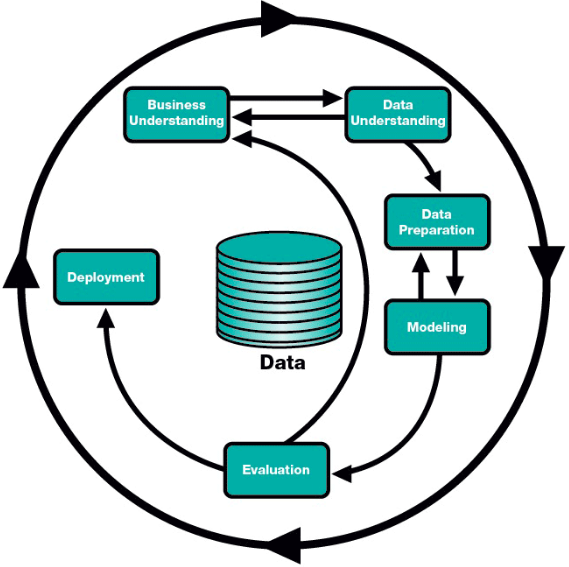
\includegraphics[scale=0.5]{img/crisp.png}
\captionof{figure}{\ac{crisp} Phasen \parencite{SmartVisionEurop}}\label{fig:crisp}
\end{center}
\textbf{Business Understanding}: diese Phase beschäftigt sich mit der Frage nach dem Ziel der Analyse. Dementsprechend, werden die Aufgaben erstellt und ein Plan festgelegt.\\
\textbf{Data Understanding}: die zweite Phase zielt darauf ab Daten zu sammeln und durch ein erstes Screening, deren Qualität festzustellen. Wie die Grafik \ref{fig:crisp} zeigt, kann dies dazu führen, die Ergebnisse aus der ersten Phase noch einmal anzupassen.\\ 
\textbf{Data Preparation}: nachdem Daten gesammelt wurden, gilt es anschließend diese für Analysen auf zubereiten. Hierbei liegt der Fokus darauf, die bestmögliche Konstruktion des finalen Datensatzes für die anschließende Modellierung zu gewinnen. Dazu ist es nötig relevante Daten auszuwählen und die Daten zu bereinigen. Dazu gehört sowohl das Entfernen und Korrigieren von Datenfehlern, als auch das Schätzen fehlender Daten durch Interpolation beispielsweise.\\
\textbf{Modeling}: diese Phase beschäftigt sich zunächst mit der Erstellung verschiedener Modelle wie zum Beispiel eines Decision Trees oder eines Neuronalen Netzes und der anschließenden Auswahl der adäquatesten Modellierungstechnik. Dazu gehört das kreieren eines Test- und eines Trainingsdatensets, womit verschiedene Modelle getestet werden können. Gegebenenfalls bedarf dies dem Wiederholen der Datenvorbereitung, um ein Datenset nochmals zu justieren.\\
\textbf{Evaluation}: währende dieser Phase wird das Modell welches die in Phase eins definierten Ziele am besten erfüllt, ausgewählt.\\
\textbf{Deployment}: in der letzten Phase werden die Ergebnisse aufbereitet und präsentiert und zusätzlich in einem Dokument festgehalten \parencite{SmartVisionEurop}.\\\\
Dieses Vorgehensmodell wurde für diese Arbeit ausgewählt, da es ein strukturiertes Vorgehen ermöglicht und dadurch die Qualität der Ergebnisse gesteigert werden kann. Das \emph{Business Understanding} besteht in dieser Arbeit darin, herauszufinden, was der momentane Stand der Forschung bezüglich Machine Learnning im Bereich Cyber Security ist. Anschließend werden bestehende Datensets untersucht, die der späteren Analyse dienen.
Um diese Daten anwenden zu können werden diese zunächst in der \emph{Data Preparation} Phase entsprechend aufbereitet. In der nächsten Phase, dem \emph{Modelling} werden diverse Algorithmen auf deren Passgenauigkeit überprüft. Anschließend wird der Algorithmus, welcher die Anforderungen am besten erfüllt, implementiert. Darüber hinaus wird das ganze Vorgehen ausführlich dokumentiert.

\chapter{IOC - Bösartiges Verhalten}\label{sec:ioc}
Die permanente Steigerung in Größe und Komplexität von Computersystemen, bietet nicht nur einen höheren Nutzen für Kunden, sondern auch mehr Angriffsfläche für Hacker. Dies erschwert die Arbeit von Sicherheitsexperten. Da es darum geht die Kompromittierung eines Systems so früh wie möglich zu erkennen, um potenziellen Schaden zu verhindern, beziehungsweise diesen so gering wie möglich zu halten, arbeiten Experten gegen die Zeit.\\
Wurde ein System Opfer eines Angriffs, gilt es dieses forensisch zu untersuchen. Normalerweise hinterlässt ein Angreifer Spuren seines Einbruchs. Die Aufgabe der IT-Security ist es, diese zu finden. Diese Hinterlassenschaften werden als \emph{\acf{ioc}} bezeichnet, also Indikatoren, welche darauf hindeuten, dass ein System kompromittiert wurde.\\
%
\ac{iocs} müssen jedoch differenziert betrachtet werden. Es gibt eindeutige Indikatoren, welche kaum einen Zweifel daran lassen, dass ein System kompromittiert wurde. Angenommen ein Sicherheitsexperte findet Schadsoftware auf einem System und stellt gleichzeitig fest, dass es zu einem Datenupload auf einen nicht identifizierbaren Server kam, welcher von der Malware initiiert wurde. In diesem Fall kann davon ausgegangen werden, dass das System tatsächlich kompromittiert wurde. Der Indikator bildet sich hierbei aus den beiden Indizien: Malware und unautorisierter Upload.\\
Des Weiteren gibt es Indikatoren welche nicht eindeutig sind. Dieses Phänomen verdeutlicht das folgende Beispiel: angenommen, auf einer Maschine werden Prozesse erkannt, welche nicht von dieser selbst gestartet wurden, sondern durch remote gesendete Befehle. Diese können durch das Windows Tool \texttt{PsExec} übermittelt worden sein. Mit Hilfe dessen, lassen sich administrative Tätigkeiten, wie beispielsweise Systemupdates oder Passwort Änderungen, anhand von Remote-Befehlen durchführen. So vorteilhaft dieses Tool in den richtigen Händen erscheint, so gefährlich ist es in den falschen. Angreifer können \texttt{PsExec} für bösartige Zwecke missbrauchen. Zwar verlangt der Remote-Zugriff eine IP-Adresse mit korrespondierenden Benutzerinformationen, diese können jedoch durch andere Arten von Angriffen beschaffen werden. Da es sich bei \texttt{PsExec} um ein legitimiertes Tool zur Systemkoordination handelt, wird es von Anti-Viren Programmen nicht erkannt. Dadurch wird die Entdeckung eines Missbrauchs deutlich erschwert. Da die Benutzerinformationen allerdings unverschlüsselt übertragen werden, können immerhin diese über Tools wie \texttt{Wireshark} oder \texttt{Tcpdump} abgefangen werden. Der Nachweis über die Nutzung dieses Tools allein reicht also nicht aus, um eine Kompromittierung annehmen zu können.
\\\\
Bei der Malware spezifischen Analyse gilt es zunächst herauszufinden, was genau passiert ist und welches Schadprogramm für den Angriff verantwortlich ist. Traditionelle Anti-Virus Programme arbeiten basierend auf Datenbanken, in welchen sie bereits bekannte Signaturen und Heuristiken anwenden, um Malware zu identifizieren. Das Problem hierbei ist, dass es für Angreifer ein leichtes ist, ihren Code zu modifizieren, um die Signatur zu verändern, wodurch das Schadprogramm nicht mehr als solches erkannt wird. Verschleierungstaktiken wie diese, lassen sich in drei Gruppen einteilen \parencite{he2017model}:
\begin{itemize}
\item \textbf{Packing} Dies Bezeichnet die Technik exekutierbare Dateien zu komprimieren. Um die komprimierte Malware zu erkennen muss diese zunächst entpackt werden. Gleichzeitig ist dies aber auch ein guter \ac{ioc}, da ausführbare Dateien im Regelfall nicht komprimiert vorliegen.
\item \textbf{Metamorphismus} Hierbei wird die Erkennung erschwert in dem der Binärcode mutiert wird. Das bedeutet, die Sequenz der Opcodes wird bei jeder Ausführung geändert.
\item \textbf{Polymorphismus} Eine polymorphe Schadsoftware generiert bei jeder Ausführung eine weitere Version der Malware, sodass eine große Anzahl an divergierender Signaturen für dasselbe Programm entstehen.
\end{itemize}
Diese Techniken erschweren das Erkennen von Malware anhand gängiger Anti-Virus Programme deutlich. Zukünftig kann Machine Learning hierbei eine große Rolle spielen. Denn wie \textcite{Han2019} bereits erfolgreich untersuchten, ist auf \ac{mlas} basierende Erkennungssoftware in der Lage, Malware trotz dieser Verschleierungstechniken zu konstatieren.
\\\\
Das Erkennen von Malware basiert im Regelfall auf der Untersuchung von \ac{pes}. Diese beinhalten ausführbare Daten im Binärformat. Dazu gehören Windows \texttt{.exe} Dateien, Objektcode und \ac{dlls}. Eine \acs{pe} ist folgendermaßen aufgebaut:
\begin{center}
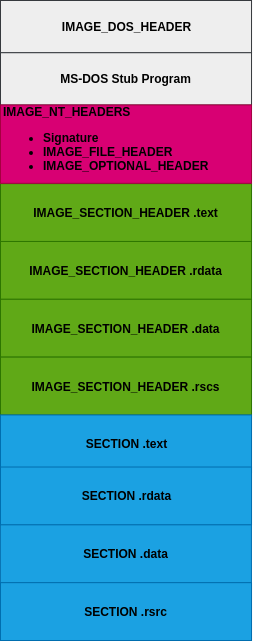
\includegraphics[scale=0.5]{img/pe.png}
\captionof{figure}{Aufbau einer \acs{pe} (eigene Darstellung)}\label{fig:pe}
\end{center}
Die in Abbildung \ref{fig:pe} grau hinterlegten Bereiche sind für die Analyse von \ac{pes} irrelevant, sie dienen unter anderem lediglich dazu, eine Fehlermeldung auszugeben, falls eine \texttt{.exe} Datei in einem Betriebssystem ausgeführt werden soll, mit welchem diese nicht kompatibel ist.\\
Der Bereich \texttt{IMAGE\_NT\_HEADERS} bietet bereits Informationen für eine Analyse. \texttt{IMAGE\_FILE\_HEADER} beinhaltet grundlegende Informationen bezüglich der Datei. Beispielsweise wann diese ausgeführt wurde, was einer Analyse sehr nützlich sein kann. Der Sektor \texttt{IMAGE\_OPTIONAL\_HEADER} ist entgegen dem was der Name vermuten lässt nicht \emph{optional}. Hier werden wichtige Informationen wie der Programmeinstiegspunkt, die Stackgröße zu Beginn sowie die Verwendung eines \ac{gui} (dt. \emph{Grafische Benutzeroberfläche}) oder einer Konsole definiert.\\
Die grün hinterlegten \texttt{IMAGE\_SECTION\_HEADER} bieten die interessantesten Informationen für eine Analyse. Diese \emph{Header} werden vom Compiler generiert und benannt, sodass der Benutzer wenig Kontrolle über die Namen hat. Dementsprechend konsistent ist die Benennung im Regelfall. Im PE-Header finden sich also relevante Informationen wie Imports, Exports, die Namen der verschiedenen Bereiche (blau hinterlegt), sowie deren Speichergröße auf der Festplatte und im \ac{ram}, sowie die Ressourcen welche von einem Programm benötigt werden.
\\\\
Grundsätzlich gibt es zwei Methoden um eine Malware Analyse durchzuführen: eine statische und eine dynamische.\\
Die Dynamische Analyse beinhaltet das Ausführen Schadhafter Programme. Dabei wird Malware in einer sicheren Umgebung ausgeführt und so dessen Verhalten analysiert. Dadurch kann im Gegensatz zur statischen Analyse die tatsächliche Verhaltensweise einer Datei untersucht werden, denn nicht jede Zeichenkette der in einer Binärdatei gefunden wird, muss zwangsläufig ausgeführt werden. Des Weiteren können Logdateien analysiert werden, welche erst durch das Ausführen eines Programms entstehen.
Dynamische Analysen werden im Regelfall in einer \emph{Sandbox}, also in einem isolierten Bereich durchgeführt, wodurch kein Schaden an der Umgebung genommen wird.
Der Nachteil dieser Analyse besteht darin, dass die Malware die virtuelle Umgebung erkennen kann und sich somit stoppt. Des Weiteren können von der Schadsoftware benötigte Registry Keys oder Dateien in der virtuellen Umgebung fehlen, sodass deren Verhalten nicht korrekt aufgezeichnet werden kann.\\\\
Eine weitere Methode zur Malware Untersuchung bietet eine statische Analyse. Hierbei werden \ac{pes} erforscht. Zunächst durchläuft potenzielle Malware diverse Virenscanner, um die Entdeckung einer bösartigen Signatur zu erhöhen.\\ 
Des Weiteren kann \emph{Hashing} zum Einsatz kommen. Dabei wird ein eindeutiger \emph{hash} generiert, welcher verwendet werden kann, um zu recherchieren, ob dieser bereits von anderen Antivirus-Dienstleistern analysiert wurde. Hashing bietet zudem den Vorteil, dass die Datei selbst noch nicht geteilt werden muss. Des Weiteren ist der Austausch eines Hashes auch um einiges schneller als der Upload einer Datei.\\
Programme verwenden Zeichenketten beispielsweise um sich mit einer URL verbinden zu können oder um Textausgaben zu drucken. Diese können einen guten Einblick über das Verhalten einzelner Programme liefern. Beispielsweise können dadurch IP Adressen für \ac{c2}-Systeme identifiziert werden, welche von Angreifern zum Verwalten von Remotesitzungen von infizierten Hosts verwendet werden.\\
Handelt es sich bei Dateien um sogenannte \emph{Packer}, also komprimierte Programme, müssen diese zunächst entpackt werden, um eine erfolgreiche Analyse durchführen zu können. Bei Dateien die relativ wenige Zeichenketten enthalten, handelt es sich meist um Packer. Wie die nachfolgende Tabelle zeigt, bietet die statische Analyse eine Vielzahl an Indikatoren, welche darauf hinweisen können, dass es sich bei der untersuchten Datei um Schadsoftware handelt.
%%%%%%%%%Table
\begin{table}[H]
\hspace{-2.8cm}
\begin{tabular}{lll}
\hline
\textbf{Ort} & \textbf{Indikator} & \textbf{Verhalten} \\ \hline
System & \begin{tabular}[c]{@{}l@{}}neue/modifizierte \\ Dateien\end{tabular} & Veränderung des Dateisystems durch Malware \\ \hline
System & Registry Einträge & Veränderung/Erstellung von Registry Keys \\ \hline
PE Header & wenige Imports & \begin{tabular}[c]{@{}l@{}}durch Packer komprimierte Dateien,\\ um die Erkennung und Analyse zu erschweren\end{tabular} \\ \hline
PE Header - Imports & \texttt{SetWindowsHookEx} & empfängt Tastatureingaben (Keylogger) \\ \hline
PE Header - Imports & \texttt{RegisterHotKey} & \begin{tabular}[c]{@{}l@{}}bestimmte Tastenkombination \\ startet Anwendung (Keylogger)\end{tabular} \\ \hline
IMAGE\_FILE\_HEADER & Kompilierungszeit & unsinnige Kompilierungszeit ist verdächtig \\ \hline
Sections & Abweichende Namen & z.B. .srtsa anstatt .data \\ \hline
SECTION .text & \begin{tabular}[c]{@{}l@{}}divergierende Speichergröße\\ von Virtual Size und Raw Size\end{tabular} & Packer extrahiert Code nach .text \\ \hline
SECTION .rsrc & eingebettetes Programm, Treiber & weitere durch Malware gestartete Aktionen \\ \hline
\end{tabular}
\caption{Auszug an, durch statische Analysen identifizierte Indikatoren für einen Malware Angriff (In Anlehnung an \textcite{Sikorski2012})}\label{table:pe}
Diese Indikatoren aus Tabelle \ref{table:pe}, sind nur ein kleiner Teil dessen, was bei einer statischen Analyse entdeckt werden kann. Dennoch wird dadurch deutlich, wie hilfreich \ac{pes} im Erkennen von Malware sein können.\\ 
Welche Features aus diesen Dateien generiert werden können, um eine aussagekräftige Untersuchung mit Hilfe von \ac{mlas} zu generieren, wird in diversen Ansätzen beschrieben, mit welchen sich das folgende Kapitel beschäftigt.
%%%%%%%%%%%%%Table
\label{tab:iocs}
\end{table}
\chapter{Analyseverfahren}
\label{sec:ba}
%\section{Machine Learning - Evaluationskriterien}
%\label{sec:mle}
Das folgende Kapitel beschäftigt sich mit Machine Learning Verfahren, welche für die Erkennung von Cyber Security Angriffen verwendet werden. Diese Verfahren wurden anhand einer umfangreichen Literaturrecherche ermittelt. Jedes Vorgehen wird auf dessen verwendete Algorithmen sowie der ausgewählten Features untersucht. Des Weiteren wird analysiert welche Evaluationskriterien verwendet wurden um die Effektivität zu messen und zu welchem Ergebnis der jeweilige Ansatz führte.\\
Das Vorgehen hierbei, orientiert sich an einem problembezogenen Ansatz. Dazu wird im Folgenden eine Übersicht darüber generiert, welche Probleme aus der Cyber Security bereits von Machine Learning Algorithmen in Angriff genommen wurden. Dies dient einer übersichtlichen Darstellung der Möglichkeiten und zeigt die Diversität auf, in welcher \ac{mlas} die Arbeit von Cyber Security Spezialisten unterstützen und verbessern können.\\\\
Zunächst werden Verfahren erläutert, welche bereits wissenschaftlich belegt wurden. Wurden, dem Ansatz entsprechende Adaptionen aus der Industrie identifiziert, wurde der jeweilige Ansatz um den industriellen erweitert.
%\section{Ansätze aus der Wissenschaft}
%\label{sec:aw}
%Das Einsatzgebiet von Machine Learning Algorithmen im Kontext von Cyber Security ist sehr breit gesteckt und reicht von der Untersuchung von Spam Profilen bei Twitter, über die Klassifizierung von Netzwerkverkehr bis hin zur Erkennung böswilliger SQL-Abfragen. Die Untersuchung dieses breit gefächerten Spektrums würde den vorgesehenen Umfang dieser Arbeit deutlich überschreiten. Infolgedessen werden lediglich Analysen dokumentiert, welche sich mit der Erkennung und Klassifizierung von Malware beschäftigen.
\section{Grundbegriffe aus der Cyber Security}
\todo[color=red!40, size=\tiny]{Angriffsvektor, Attacken erklären}
\section{Grundbegriffe des maschinellen Lernens}
\todo[color=red!40, size=\tiny]{Leistungsindikatoren, Algorithmen erklären}
\section{Angewandte Ansätze}
Für die Recherche wurden alle Verfahren in einem Zeitraum von 2015 bis heute berücksichtigt. Diese Periode wurde gewählt, da sich die Zahl der Cyberangriffe, sowie die zur Verfügung stehende Schadsoftware bereits innerhalb weniger Jahre deutlich vermehrt beziehungsweise verändert. Somit soll verhindert werden veraltete Angriffsvektoren zu analysieren, welche bereits von moderneren überholt wurden. Zusätzlich gibt es bereits vergleichbare Arbeiten aus dem Jahr 2016 \parencite[s.][]{Buczak2016}, in welchem Machine Learning Ansätze vor dieser Zeit analysiert werden.\\
In der folgenden Auflistung wird die Bezeichnung \emph{Erkennung} für binäre Klassifikation verwendet. Beispielsweise, wenn sich ein Ansatz darauf beschränkt Daten entweder in die Rubrik A \emph{bösartig} oder in die Rubrik B \emph{gutartig} zu klassifizieren.\\
Erfolgt in einem Analyseverfahren eine Einteilung in mehrere Klassen (mehr als zwei), wird nachfolgend der Begriff 
\emph{Klassifizierung} verwendet.
\\\\
%%%%%%%%%%%%%%%%%%%%%%%%%%%%%%%%%%%%%%%%%%%%%%%%%%%%%%%%%%%%%%%%%%%%%%%%%%%%%%
%wenn binäre Klassifikation:
%%%%"Erkennung von..."
%Wenn Multiclass Klassifizierung:
%%%%"Klassifizierung von..."
%Ansonsten "..Erkennung" etc.
%%%%%%%%%%%%%%%%%%%%%%%%%%%%%%%%%%%%%%%%%%%%%%%%%%%%%%%%%%%%%%%%%%%%%%%%%%%%%%
\subsection{Erkennung von Malware - Hybride Analyse (2015)}
Im Jahr \citeyear{Shijo2015} haben \textcite{Shijo2015} einen, auf zwei Analysen basierenden, Ansatz gewählt, um Malware zu erkennen. Dabei vermischten sie die statische Analyse mit der dynamischen, um so einen hybriden Ansatz zu erreichen. Zum einen verwendeten sie ein statisches Analyseverfahren bei dem sie \emph{Printable Strings}, also nicht kodierte Zeichenfolgen wie z. B. \emph{FindFirstFile} aus Binärdateien extrahierten. Zum anderen konfigurierten sie eine Cuckoo Sandbox, in der sie Schadsoftware ausführten und deren API Aufrufe in einer Protokolldatei speicherten.\\
Sie untersuchten die Ähnlichkeit in API-Aufrufsequenzen anhand von n-Gramm-basierter Ähnlichkeitsmessung. 
Als Features dienten Tri- und Tetragramme ab einer gewissen Häufigkeit, sowie PrintableStrings ab einer Häufigkeit von zwei.
Für die Klassifizierung wurden die Algorithmen \ac{rf} und \ac{svm} verwendet.
Es wurden jeweils beide Ansätze separat, sowie in Kombination getestet. Analysen mit \ac{svm} erzielten eine Genauigkeit von 95.88 \% für die statische Analyse und 97.16 \% für die dynamische Analyse und waren somit erfolgreicher, als Untersuchungen mit Random Forest. Die besten Ergebnisse erzielte der hybride Ansatz mit \ac{svm} mit einer Genauigkeit von 98.71 \% und der geringsten \ac{fpr} von 0.026.\\
Die Forschung von \textcite{Shijo2015} zeigt also, dass mit den von ihnen gewählte Features, mit einem hybriden Ansatz, deutlich genauere Aussagen, als mit rein statischen oder rein dynamischen Analysen, getroffen werden können.

%
\subsection{Erkennung von Malware - Statische Analyse (2016)}
\textcite{More2016} untersuchten EXE-Dateien auf Schadsoftware. Dazu konvertierten sie die Dateien zunächst in \ac{opcode}, also in den Teil der Maschinensprachanweisung der die auszuführenden Operationen angibt, z.B. \texttt{55 8B EC 83 EC 5C 83 7D 0C 0F 74 2B 83 7D 0C 46}. Das ausgewählte Feature Datenset wurde anschließend nochmals zu einer \ac{arff} Datei konvertiert, um die Datei nachfolgend mit der Machine Learning Software Weka bearbeiten zu können. 
In Weka wurden die Algorithmen JRip, C4.5 und \ac{ibk} verwendet. Wobei es sich bei JRip und C4.5 um \ac{dt} und bei \ac{ibk} um \ac{knn} Implementierungen handelt. Um die Erkennungsgenauigkeit zu erhöhen, wurden nicht nur die einzelnen Algorithmen, sondern ein Klassifikatorensemble angewandt, um Methoden wie Mehrheitsvoting, Veto-Voting und vertrauensbasiertes Veto-Voting verwenden zu können. Ersteres folgt demokratischen Regeln, das heißt, die Klasse mit den meisten Stimmen ist das Ergebnis. Veto-Voting hingehen basiert auf Annahmen über die Wahl der anderen Algorithmen. Vertrauensbasiertes Veto-Voting ergänzt voriges Voting um eine Vertrauensberechnung, wodurch jedem Algorithmus ein bestimmtes Vertrauensniveau zugeteilt wird. Weiterführende Informationen bezüglich dieser Methoden können \textcite{shahzad2013comparative} entnommen werden. \\
\textcite{More2016} konnten zeigen, dass durch die Verwendung von Veto-Voting eine Genauigkeit von 80.7 \% erzielt werden kann. Im Vergleich dazu, lag das beste Ergebnis, welches durch singulären Algorithmeneinsatz von \ac{ibk} erzielt wurde, bei einer Genauigkeit von nur 73.5 \%.\\\\
Dieses Ergebnis stützt die These von \textcite{Shijo2015} aus dem Jahr zuvor, welche zeigten, dass ein nicht-hybrider Ansatz weniger genau ist, als einer, der die statische und die dynamische miteinander verknüpft.
\subsection{Erkennung bösartiger XML-basierter Office Dokumente(2016)}
Durch das neue Dateiformat, welches  2007 auf den Markt gebracht hat, sollten Sicherheitslücken geschlossen werden.
Das Binärformat wurde durch ein	XML basiertes Dateiformat ersetzt. Dadurch werden neue digitale Funktionen unterstützt, sowie vertrauensbasierte Bereiche geschaffen, welche das Format weniger riskikoreich gestalten sollen. Dennoch können Attacken gegen XML-basierte Office Dokumente gestartet werden. Zu den möglichen Angriffsvektoren zählen beispielsweise macrobasierte Attacken. Durch den Missbrauch von \ac{vba} kann die zugehörige shell gestartet werden, um willkürliche Kommandos zu senden. Außerdem können externe Bibliotheken sowie Programme aufgerufen werden, welche Schaden verursachen können. Eine weitere Bedrohung durch den Gebrauch von Macros bildet die Fähigkeit dieser, bösartige Dateien aus dem Internet herunterzuladen.\\
\textcite{Cohen2016} haben in ihrer Arbeit diese Art von Angriffsvektoren untersucht, um eine Infizierung durch bösartige Macros frühzeitig zu erkennen. Dazu haben sie zunächst Office Dokumente in eine Liste von Pfaden konvertiert. Diese dienen der Analyse als Features.
\begin{center}
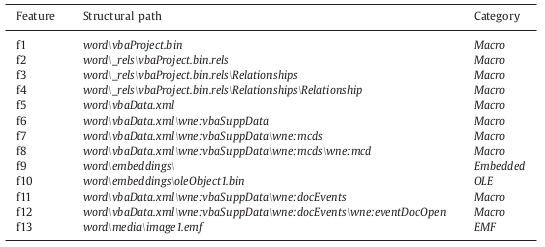
\includegraphics[scale=0.6]{img/pfade.png}
\captionof{figure}{Features als Pfade dargestellt \parencite{Cohen2016}}\label{fig:pe}
\end{center}
Dadurch wurde jedoch eine so hohe Anzahl an Features generiert, dass die Untersuchung mit verschiedenen Datensets durchgeführt wurde, welche Top Features von 10 bis 2000 beinhalteten. Um die Feature-Repräsentation, also das Vorhandensein bzw. die Wichtigkeit von Features zu bestimmen, wurden zwei Verfahren angewandt. Zum einen ein binäres Verfahren, welches lediglich die Ab-, respektive Anwesenheit eines Features misst und zum anderen wurde das statistische Verfahren \ac{tfidf} verwendet, um die Wichtigkeit eines Terms in Bezug auf ein Dokument zu bestimmen. Anschließend wurden die Daten mit folgenden Algorithmen untersucht: J48, \ac{rf}, \ac{lr}, \ac{nb}, \ac{bn}, \ac{lb}, \ac{smo}, Bagging und \ac{ab}. \\\\
Wie die Ergebnisse zeigen, erzielt das Datenset mit den Top 200 Features, welches mit Random Forest analysiert wurde die besten Werte mit einem F-measure von 0.66.
Wie sich demonstrieren ließ, ist es möglich bösartige Office Dokumente durch eine Analyse deren Pfade zu erkennen. 
Die Untersuchung beschränkt sich jedoch auf direkte Gefahren innerhalb von Dokumenten. Indirekte Gefahren, wie etwa die durch weiterführende Links, wurden in dieser Forschungsarbeit nicht berücksichtigt.
\subsection{Erkennung bösartiger HTTP-Anfragen (2016)}\label{csic}
\textcite{Pham2016} haben in ihrer Arbeit ein \ac{ids} für \ac{http} - Anfragen entwickelt. Dazu nutzen sie ein von ihnen entwickeltes Modul, um Netzwerkpakete zu erfassen. Dieses Modul basiert auf derselben Erfassungstechnik die \texttt{Wireshark} verwendet. Um ein geeignetes Model zu zu evaluieren, welches es ermöglicht die Pakete in Echtzeit zu klassifizieren, wurden diverse \ac{mlas} anhand des CSIC 2010 HTTP Datensets von \textcite{csic} getestet. Dieses besteht aus 223585 Daten die entweder als \emph{normal} oder \emph{anomal} gelabelt sind. Es enthält Attacken wie SQL-Injections, Buffer Overflow und \ac{xss}. \textcite{Pham2016} trainierten und testeten die Daten mit den Algorithmen Decision Tree, Random Forest, AdaBoost, Logistic Regression und dem  SGDClassifier. Als Evaluationsmethode wurden Precision, Recall und F-measure verwendet. Den höchsten dieser Werte erzielte die Logistic Regression Methode mit einem F1-measure von 0.96 for abnormen und 95.82 für normalen Verkehr. Zukünftig sollen diese Ergebnisse an Paketen, welche durch das eigens entwickelte Modul der Forscher erfasst wurden, evaluiert werden.
%
\subsection{Klassifizierung von Netzwerkattacken (2017)}\label{yin}
\textcite{Yin2017} implementierten ein \ac{ids}, für welches sie \ac{rnns} verwendeten. Zusätzlich wurde die Leistung des Models bei binärer als auch bei Multi-Klassen Klassifikation untersucht. Um die Effizienz zu prüfen, wurde ferner ein Vergleich mit diversen \ac{mlas} gezogen. Die Analyse basiert auf dem NSL-KDD Datenset aus dem Jahr 2009 \parencite{Cybersecurity}. Dieses beinhaltet neben dem normalen Netzwerkverkehr, Daten zu vier verschiedenen Angriffstypen die da wären: \ac{dos}, \ac{r2l}, \ac{u2r} und Probe Attacken. Das Datenset besteht aus 41 Features. Um Vergleiche mit anderen \ac{mlas} herzustellen, wurden parallel Experimente mit \ac{ann}, \ac{rf}, \ac{nb}, \ac{mlp}, \ac{svm}, J48, Random Tree und \ac{nbt} für die binäre Klassifikation durchgeführt. Auf dieselbe Weise wurde die Multi-Klassen Klassifikation überprüft. Als Qualitätsmerkmal der Ergebnisse wurde der Wert \emph{Accuracy} gewählt, welcher die Genauigkeit der Analyse wider spiegelt. Dieser Wert basiert auf dem Prozentsatz der korrekt klassifizierten Daten im Vergleich zur Gesamtheit der Daten. Das Ergebnis zeigt, dass \ac{rnns} eine qualitativ hochwertigere Analyse produzieren als die zu verglichenen \ac{mlas}. Bei der binären Klassifikation des Testsets erzielte auf \ac{rnns} basierende Untersuchungen eine Genauigkeit von 83.28\% gefolgt von \ac{nbt} mit 82.02\%. Bei der Klassifizierung in fünf Klassen erreichte das \ac{rnn} mit 81.29\% ebenfalls ein besseres Ergebnis als die restlichen Algorithmen. Jedoch fanden \textcite{Yin2017} heraus, dass \ac{rnns} deutlich mehr Zeit für das Training beanspruchen, dieses Problem soll zukünftig durch Nutzung der \ac{gpu} beschleunigt werden.
%
\subsection{Erkennung von Ransomware - Dynamische Analyse (2017)}
\textcite{Maniath2018} haben eine dynamische Analyse entwickelt um \emph{Ransomware} anhand von API Aufrufen zu klassifizieren. Ransomware beschreibt eine Art Schadprogramm, welche dem Benutzer Ressourcen entzieht und eine Lösegeldsumme verlangt um diese wieder verfügbar zu machen. Um die Aufrufe zu extrahieren verwendeten die Forscher die dafür entwickelte Umgebung von Cuckoo Sandbox. Dadurch konnten die Schadprogramme in einer Umgebung ausgeführt werden ohne Schaden zu erzeugen. Die Anwendung erfasst alle API Aufrufe und speichert diese in einer \texttt{.json} Datei. Für die Analyse wurden 157 schadhafte Dateien aus nicht näher beschriebenen Onlinequellen verwendet. Dabei konnten 239 Aufrufe extrahiert werden, welche der Untersuchung als Features dienten. Um eine einheitliche Länge dieser zu gewährleisten, wurden die einzelnen Aufrufe entsprechend der längsten Sequenz mit Nullen aufgefüllt. Anschließend wurden die Daten entweder mit 0 für \emph{gutartig} oder mit 1 für \emph{ransomware} gelabelt. Anhand dieser Daten wurde ein \ac{lstm} Netzwerk trainiert. Nach einer Trainingszeit von zwei Stunden erreichte das Model eine Genauigkeit von 96.67\% bei der Analyse der Testdaten. Die komplette Prozess einschließlich der Gewinnung der API Sequenzen dauerte allerdings 56 Stunden, was in Anbetracht der geringen Menge an Datensätzen doch sehr nachteilig ist.
%
\subsection{Erkennung von Malware - Imageanalyse (2017)}
Eine potenziell schnellere Methode um Malware zu erkennen, entwickelten \textcite{8190895} anhand einer Image Analyse. Dazu generieren sie Bilder von ausführbaren Dateien. Dabei hat jedes Pixel einen Wert zwischen 0 und 255. Um aus einer Datei ein Bild zu erhalten, wird jedes Byte eingelesen und zu einer Ganzzahl konvertiert die einem Pixel entspricht. Dadurch entstehen 256x256 Bilder. Da dadurch während einer Analyse der Speicher zur Neige geht wurden die Daten auf 32x32 reduziert. Die dadurch generierten Bilder dienen der Analyse mit einem \ac{cnn} als Features. Die 2000 dafür verwendeten Schadprogramme, stammen aus einem koreanischen Cyber Security Forschungszentrum. Als Metrik zur Überprüfung der Genauigkeit wurde hier ebenfalls die Genauigkeit gewählt, welche sich auf 95.66\% beläuft.\\
Bedauerlicherweise haben \textcite{8190895} nicht erwähnt in welcher Geschwindigkeit sie ihre Analyse durchführen konnten. In Anbetracht der von ihnen aufgestellten These - Imageanalysen seien viel schneller als statische und dynamische Analysen - wäre dies ein interessantes Detail gewesen.

%
\subsection{Erkennung böswilliger MS Office Dateien (2017)}
\textcite{Bearden2018} konzentrierten sich in ihrer Forschung darauf eine Methode zu entwickeln, mit welcher sich Microsoft Office Dokumente anhand ihrer Macros nach \emph{gutartig} und \emph{bösartig} klassifizieren lassen. Dazu untersuchten sie 158 Dateien, von welchen 40 schadhaft waren. Dokumente die Macros enthalten, beinhalten nicht nur \ac{vba} Code sondern auch \emph{p-code}. Dabei handelt es sich um Assembler-Code, welcher vom \ac{vba}-Interpreter generiert wird, nachdem der Code einmal ausgeführt wurde \parencite{Bearden2018}. Diese Codes dienten der Analyse mit \ac{knn} als Features. Die Effizienz wurde, wie die beiden zuletzt erläuterten Ansätze, anhand der Genauigkeit gemessen. Es wurden verschiedene Experimente mit unterschiedlichen \emph{K} und \emph{L} durchgeführt, wobei \emph{K} die Anzahl an Clustern und \emph{L} die Anzahl der besten Features impliziert. Den besten Wert erzielte eine Kombination mit K=3 und den Top 75 Features mit einer Genauigkeit von 96.3\%.\\Es wurde ausschließlich ein Algorithmus getestet, da die Intention der Forschung darin bestand , einen \emph{Proof of concept} für die Erkennung bösartiger Macros anhand von p-codes bereitzustellen. Der Vorteil den \textcite{Bearden2018} mit ihrer Forschung geschaffen haben, besteht darin, dass potenziell bösartige Dateien nicht geöffnet werden müssen, bevor sie analysiert werden können. Jedoch weisen auch sie auf den Mangel an adäquaten Trainingsdaten hin, welchen es zukünftig zu beheben gilt.
%
\subsection{Klassifizierung von \acs{ddos} Attacken (2017)}
Bereits seit den 80er Jahren gibt es \ac{dos} Attacken, welche Netzwerk Ressourcen erschöpfen und dadurch die Verfügbarkeit von Services blockieren. Es gibt zwei Arten diese Attacken zu erkennen: Zielseitige Verteidigung und Quellenseitige Verteidigung\parencite{He2017}. Die Zielseitige Erkennung hat den Nachteil, dass Attacken erst entdeckt werden nachdem sie bereits beim Opfersystem ankamen. \textcite{He2017} forschen an einem pro aktiven Ansatz, bei dem die Erkennung auf der Quellenseite erfolgen soll, wodurch Angriffe auf mehrere Systeme verhindert werden können. Dabei konzentrieren sie sich auf vier gängige \ac{ddos} Angriffe aus der Cloud: \ac{ssh} brute-force Attacken, \ac{icmp} flooding Attacken, \ac{dns} reflection Attacken und \ac{tcp} \ac{syn} Attacken. Als Feature für \ac{ssh} brute-force Attacken dient die Anzahl an Diffie-Hellman Schlüsselaustausche, da dieser Wert während einer solchen Attacke steigt \parencite{He2017}. Als Feature für \ac{dns} reflection Attacken wurde das Verhältnis von eingehenden und ausgehenden \ac{dns}-Paketen gewählt, da bei einer Attacke mehr Anfragen als Antworten gesendet werden. Die \ac{icmp} Paketrate wurde als Feature für \ac{icmp} flooding Attacken gewählt, da bei normalem Verkehr eine geringere Anzahl dieser Pakete vorhanden ist. Um \ac{tcp}-\ac{syn} Attacken zu identifizieren, wurde das \ac{syn}/\ac{ack} Verhältnis als Feature gewählt, da während einer solchen Attacke mehr \ac{syn} Tags als \ac{ack} Tags in den Paketen zu finden sind. Für das Experiment wurde der Netzwerkverkehr 9 Stunden lang verfolgt und anschließend mit den Algorithmen \ac{lr}, \ac{svm}, \ac{dt}, \ac{nb}, \ac{rf}, k-means und \ac{gmm} klassifiziert. Zur Evaluation dienten die Metriken: Precision, Genauigkeit, Recall und F1-measure. Das beste Ergebnis mit einem F1-measure von 0.9975 und einer Genauigkeit von 99.73\% konnte mit \ac{svm} erzielt werden.
Durch diesen vielversprechenden Ansatz sollen zukünftig weitere \ac{ddos} Attacken pro aktiv erkannt werden.
%
\subsection{Schwachstellen Scanner für Web Applikationen (2017)}
Um Schwachstellen in Web Applikationen zu finden, wurde bei diesem Ansatz ein System namens \ac{btb} entwickelt \parencite{VidyavardhakaCollegeofEngineering2017}. Dieser Schwachstellenscanner überprüft Websites auf potenzielle Angriffsvektoren und liefert gleichzeitig Lösungen, um diese zu beheben. Zunächst überträgt der Bot alle Seiten einer Webapplikation und sucht innerhalb dieser nach ausnutzbaren Schwachstellen. Das Überprüfen basiert auf dem Ausführen von Payloads für gefundene Konflikte. Beispielsweise können Seiten auf SQL-Injections und \ac{xss} Attacken überprüft werden, in dem adäquate Payloads ausgeführt werden. Anschließend werden Code Vorschläge geliefert, welche die gefundenen Schwachstellen schließen sollen. Das Ergebnis des Scans, sowie die Verbesserungsvorschläge basieren auf Machine Learning. Nach dem Scan werden die Daten an einen zentralisierten Server geschickt, auf welchem eine \ac{svm} Informationen zu Schwachstellen analysiert und entsprechende Vorschläge für Payloads und gleichzeitig verfügbare Patches liefert. Um die Effizienz dieses Systems zu messen, wurde ein Leistungsfaktor \emph{E} berechnet. Dieser setzt sich aus der benötigten Zeit für den ersten Scan sowie dem des letzten Scans zusammen. Wie Experimente zeigen, nimmt die Dauer der Scans mit \ac{btb} ab, während Überprüfungen mit Scannern ohne Machine Learning Komponenten in der Dauer konstant bleiben.\\
Mit dieser Forschung wurde gezeigt, dass durch Machine Learning schnellere Ergebnisse bereitgestellt werden können.
%
\subsection{Erkennung von Malware anhand von PE-Header (2017)}
\textcite{Raff2017} verzichten in ihrem Ansatz auf explizite Feature Konstruktionen und zeigen, dass Malware anhand von Bytes von Neuronalen Netzen erkannt werden kann. 
Für diese Analyse untersuchten sie zwei verschiedene Ansätze, ein \ac{fcn} und ein \ac{rnn}, bei welchem sie sich für das \ac{lstm} Model entschieden. Gerade deshalb war es nötig sich bei der Analyse auf den Header der \ac{pes} zu konzentrieren, da \ac{lstm} Modelle für die Berechnung aller Daten enorm viel Zeit und Ressourcen in Anspruch nehmen würden \parencite{Raff2017}. Die dabei verwendeten Features bestehen aus 328 geordneten Bytes.
Zusätzlich wurden Modelle entwickelt um Vergleiche mit den Ergebnissen der Neuronalen Netze anzustellen. Dazu gehören \ac{et}, \ac{rf} und \ac{lr}. Um die Vorhersagen zu evaluieren wurden die Metriken Genauigkeit sowie \ac{auc} verwendet. Entsprechende Daten sammelten die Forscher sowohl bei \emph{VirusShare} als auch bei \emph{OpenMalware}. Wie die Ergebnisse zeigen liegt der vielversprechendste Ansatz in \ac{fcn} mit einer Genauigkeit von 89.9\% gefolgt von dem \ac{rnn} \ac{lstm} mit 79.7\%.\\
Durch diese Forschung zeigen die Autoren das Potenzial Neuronaler Netze im Erkennen von Schadsoftware lediglich anhand von rohen Bytes. Dies impliziert nicht nur eine enorme Zeit sondern auch eine bemerkenswerte Ressourcen Einsparung.
%
\subsection{Erkennung von Malware anhand von PE-Header mit erweitertem  Feature-Set (2017)}
Im Gegensatz zu dem zuvor erläuterten Ansatz  von \textcite{Raff2017}, verwenden \textcite{Kumar2017} ein erweitertes Feature Set für ihre Analyse. Dieses setzt sich aus \emph{rohen} Features, wie beispielsweise der Anzahl der \texttt{FILE\_HEADER}-Abschnitte, und \emph{abgeleiteten} Features zusammen. Bei Letzterem handelt es sich um Werte, die durch den Abgleich von Feature-Werten mit vorab definierten Regeln entstehen. Beispielsweise könnte der Wert der Kompilierungszeit, bei welchem es sich um eine Ganzzahl, die die vergangene Zeit seit 1969 in Sekunden angibt, handelt, allein wenig Aussagekraft besitzen \parencite{Kumar2017}. Deswegen wird die Zahl in ein Datumsformat konvertiert und mit einem bestimmten Gültigkeitsbereich verglichen. Dadurch ergibt sich ein boolescher Wert, welcher in die Analyse mit einfließt. \textcite{Kumar2017} verwenden insgesamt 11 abgeleitete und 55 rohe Features. Für ihre Analyse sammelten die Autoren bösartige Dateien bei \emph{VirusShare} und \emph{download.cnet}. Es wurden Experimente anhand  rohen Feature Sets als auch anhand eines integrierten Feature Sets (welches aus rohen und abgeleiteten Features besteht) mit \ac{lr}, \ac{lda}, \ac{rf}, \ac{dt}, \ac{nb} und \ac{knn} durchgeführt. Als Evaluationsmetriken wurden Genauigkeit, Precision, Recall und der F1-measure verwendet. Bis auf \ac{knn} erzielten alle Algorithmen ein besseres Ergebnis, wenn das integrierte Feature Set verwendet wurde. Den besten Wert erreicht \ac{rf} mit einer Genauigkeit von 89.23\% und einem F1-measure von 0.90. \\
Diese Ergebnisse erzielen somit eine höhere Genauigkeit als die der Untersuchungen von \textcite{Raff2017}, jedoch ist eine weitaus intensivere Vorarbeit zu leisten.
%
\subsection{Erkennung von Exfiltration und \acs{cc}Tunnels (2017)}
\textcite{Das2018} entwickelten ein auf Machine Learning basierendes System um die Exfiltration von Daten eines kompromittierten Systems, sowie den Aufbau eines \ac{cc}-Servers zu erkennen. Um Daten zu exfiltrieren kann Schadsoftware \ac{dns} Abfragen nutzen. Dazu kodiert und/oder komprimiert sie die zu versendenden Informationen zunächst. Anschließend kann die daraus entstandene Zeichenkette als Subdomain einer \ac{dns} Abfrage angehängt werden.\\
Über \ac{dns} TXT-Records können Texte anstatt einer IP Adresse an einen Benutzer gesendet werden. Angreifer können diese Funktion nutzen, um einen Tunnel zum Senden von Anweisungen oder zum Öffnen einer Sitzung einzurichten.
Bei der Exfiltration gehen die Autoren davon aus, dass eine kodierte Subdomain ein Indiz hierfür ist, weshalb diese Zeichenkette analysiert wird. Zunächst generieren sie aus dieser acht Features wie beispielsweise dem Verhältnis der Anzahl an Ziffern zum Rest der Elemente. Das von \textcite{Das2018} entworfene Model basiert auf \acl{lr} und erreicht einen F1-measure von 0.96.\\
Für die Klassifizierung von TXT-Records wählten sie einen \emph{unsupervised learning} Ansatz, d.h. das Modell arbeitete mit einem ungelabelten Datenset. Für die Analyse verwendeten sie zehn Features, unter anderem die Anzahl der Groß- sowie der Kleinbuchstaben, Punkte oder Unterstriche sowie die Anzahl von Ziffern. Dadurch konnten von 2356 bösartigen TXT-Records 2160 von ihrem Modell identifiziert werden.
%
\subsection{Erkennung bösartiger PowerShell-Befehle (2018)}
\textcite{Hendler2018} untersuchten in ihrer Forschung von 2018 bösartige PowerShell Befehle. Dazu analysierten sie ein Datenset welches aus über 66.000 Befehlen bestand. Die hierbei verwendeten bösartigen Befehle stammen von Microsoft-Sicherheitsexperten.  Das Datenset musste zunächst vorverarbeitet werden. Dazu wurden beispielsweise kodierte Befehle zunächst dekodiert, Leerzeichen wurden entfernt und Nummern durch ein Sternchen (*) ersetzt. Anschließend wurden die Daten sowohl mit einem \ac{cnn} als auch mit einem auf \ac{nlp} basierenden Detektoren untersucht. Das beste Ergebnis erzielte allerdings ein Ensemble-Detektor, der einen \ac{nlp}-basierten Klassifikator mit einem \ac{cnn}-basierten kombiniert. Dieser erzielte eine \ac{tpr} von 0.92.\\
Da das verwendete Datenset nicht einsehbar ist, bleibt hier unklar, was einen PowerShell Befehl bösartig macht. Da viele Befehle von Administratoren als auch von Angreifern gleichermaßen genutzt werden, wäre dies ein interessantes Detail gewesen.
%
\subsection{Klassifizierung von Netzwerkverkehr in 5 Klassen (2018)}\label{ding}
\textcite{Ding2018} wählten den Ansatz eines \ac{cnn} um ein \ac{ids} aufzubauen, da laut ihnen Systeme, welche mit traditionellen \ac{mlas} arbeiten nicht explizit und nicht zuverlässig genug sind. Um diese These zu verifizieren verglichen sie die Ergebnisse des \ac{cnn} mit traditionellen Algorithmen wie \ac{rf} und \ac{svm} und Deep Learning Methoden wie \ac{dbn} und \ac{lstm}. Wie \textcite{Yin2017}, verwendeten sie das NSL-KDD Datenset, welche dieses bereits mit \ac{rnn} analysierten. Auch \textcite{Ding2018} wählten als Leistungsindikator die Genauigkeit, sowie die \ac{tpr} und die \ac{fpr}. Tatsächlich lag die Genauigkeit des \ac{cnn} mit 80.13\% deutlich über der, der traditionellen als auch der Deep Learning Methoden. Jedoch erzielten \textcite{Yin2017} mit ihrem \ac{rnn} eine um knapp 2\% bessere Analyse bei der Klassifikation des Netzwerkverkehrs in 5 Klassen. Da laut \textcite{Yin2017} \ac{rnns} deutlich mehr Trainingszeit benötigen als traditionelle \ac{mlas}, wäre es interessant zu vergleichen gewesen, wie sich die Trainingszeit bei dem von \textcite{Ding2018} entwickelten \ac{cnn} verhielt. Leider ist dieses Detail in der Arbeit nicht dokumentiert.
%
\subsection{Anomalieerkennung anhand von Systemprotokollen (2018)}\label{brown}
Computersysteme produzieren täglich Terabytes an Daten, welche unmöglich manuell inspiziert werden können. Dadurch scheint dies ein für \ac{mlas} prädestinierter Use Case zu sein. \textcite{Brown2018} untersuchten in ihrer Arbeit die Analysefähigkeit von \ac{rnns} in Systemprotokollen. Da die Autoren auf unbeaufsichtigte Lernmethoden setzen, kann auf die zeitaufwändige Beschaffung von gelabelten Daten verzichtet werden. Um das von ihnen entwickelte Modell zu evaluieren, verwendeten sie das \ac{lanl} \parencite{akent-2015-enterprise-data}, welches Host Ereignisse protokolliert. Dieses besteht aus über einer Milliarde Protokollzeilen, welche jeweils 21 Features beinhalten. Von diesen verwendeten die Autoren lediglich acht für ihre Analyse und reduzierten den Datensatz auf 14 Millionen Protokollzeilen, da sie nur mehr zwei Tage der Aufzeichnungen berücksichtigten. Um die Ergebnisse zu überprüfen verwendeten sie die \ac{aucroc}. Dieser ergab einen \ac{auc} Wert von 0.976 und zeigt deutlich das die Analyse mit unbeaufsichtigten \ac{rnns} ein hohes Potenziell für die Untersuchung von Logdateien besitzt.
%
\subsection{Erkennung von bösartigem Netzwerkverkehr (2018)}\label{iscx1}
\textcite{Aldwairi2018} verwendeten in ihrer Arbeit eine \ac{rbm} um Netzwerkverkehr binär nach \emph{normal} oder \emph{anormal} zu klassifizieren. Im Vergleich zu Neuronalen Netzen die aus \emph{Input}, \emph{hidden} und \emph{output} Schicht bestehen, enthält eine \ac{rbm} lediglich die erste beiden Schichten. Im Vergleich zu \textcite{Yin2017} und \textcite{Ding2018}, verwenden \textcite{Aldwairi2018} nicht das NSL-KDD Datenset, sondern das ISCX Datenset \parencite{shiravi2012toward}, in welchem Netzwerkverkehr aus dem Jahr 2012 aufgezeichnet wurde. Für ihre Analyse verwendeten die Forscher 16 Features die verschiedene Merkmale des Netzwerkverkehrs beschreiben.  Um die Leistung der \ac{rbm} zu evaluieren verwendeten auch sie den Leistungsindikator der Genauigkeit und erzielten dabei einen Wert von 89\%. Außerdem vermerkten sie eine \ac{tpr} von 88.4\% und eine \ac{fnr} von 88.8\%. Da \textcite{Aldwairi2018} lediglich eine zweischichtige \ac{rbm} verwendeten, wäre es interessant weitere Experimente mit so genannten \ac{drbms}, welche aus mehreren Schichten bestehen, durchzuführen.
%
\subsection{Erkennung von Botnetzen (2018)}\label{ctu}
Botnetze sind eine Sammlung an kompromittierten, miteinander verbundenen Maschinen, die durch einen Master gesteuert werden. Diese Netze können Bedrohungen wie \ac{dos} Attacken, Spamming oder Datendiebstahl auslösen. Laut \textcite{leonard2009framework} besteht der Lebenszyklus eines Botnetzes aus vier Phasen: Formation, \ac{cc}, Attacke, post Attack-Phase. Um diese Art von bösartigem Verhalten zu Analysieren, entwickelten \textcite{Mathur2018} ein Modell, welches Botnetze in den ersten beiden dieser Phasen erkennt. Um Attacken so früh wie möglich zu erkennen, setzen die Forscher auf ein zeitsparendes Analyseverfahren bei welchem lediglich der Header von \ac{tcp}/\ac{udp}-Paketen untersucht wird. Um entsprechende Daten zu generieren wurde Netzwerkverkehr von Linux als auch von Windows Systemen erfasst. Zusätzlich verwendeten die Forscher das CTU-13 \parencite{garcia2014empirical}, sowie das ISOT \parencite{isot} Datenset. Insgesamt wurden 11 Features wie beispielsweise Fließdauer, Ziel und Quell IP Adresse sowie das zu verwendete Protokoll verwendet. Bei der Analyse kamen die Algorithmen \ac{lr}, Random SubSpace, Randomizable Filtered Classifier, MultiClass Classifier und Random Committee zum Einsatz. Dabei erzielte der MultiClass Classifier eine Genauigkeit von 98.4\% sowie eine \ac{fpr} von lediglich 0.004 in einer Zeit von 0.03s. Somit beweisen \textcite{Mathur2018} einen praktikablen Ansatz im Erkennen von Botnetzen, allerdings bemängeln sie die Genauigkeit bei einem exponentiellen Anstieg von Netzwerkverkehrsdaten, sie empfehlen daher für eine größere Menge an Daten neuronale Netze zur Erkennung zu verwenden.
%
\subsection{Klassifizierung von Microsoft Malware (2018)}\label{sabar}
\textcite{Sabar2018} setzen bei der Erkennung von Malware auf \ac{svm}. Jedoch optimieren sie deren Konfiguration durch Verwendung von hyper Heuristiken. Dabei handelt es sich um eine Suchmethode welche unter diversen Heuristiken auswählt und diese gegebenenfalls miteinander kombiniert, um eine bestmögliche problemspezifische Konfiguration zu gewährleisten. Die Daten für die Analyse entnahmen sie der Microsoft Kaggle Challenge von 2015 \parencite{Kaggle}, bei welcher es 500 GB Schadsoftware Dateien in neun verschiedene Klassen zu klassifizieren galt. Zusätzlich verwendeten sie das NSL-KDD Datenset. Um den von ihnen entwickelten Ansatz zu evaluieren, analysierten sie die Datensätze zusätzlich mit den Algorithmen \ac{gnbt}, \ac{fc} und \ac{dt}. Als Leistungsindikatoren wählten sie die Genauigkeit sowie den \emph{logloss} (dt. Logarithmischer Verlust), welcher die Leistung eines Modells misst, dessen Ausgabe einen Wahrscheinlichkeitswert zwischen 0 und 1 annehmen kann. Dabei steigt der Wert wenn die Annahme von dem tatsächlichen Wert abweicht und sinkt wenn er mit diesem übereinstimmt. Dementsprechend ist ein Wert welcher gegen 0 strebt wünschenswert. Tatsächlich erzielte der Ansatz von \textcite{Sabar2018} den niedrigsten logloss mit einem Wert von 0.0031 \footnote{Das Gewinner Team der Kaggle Challenge erzielte einen logloss von 0.0028 \parencite{leader}.}. Des Weiteren konnte ebenfalls damit die höchste Genauigkeit von 85.69\% erreicht werden. Dadurch konnten die Forscher die Effektivität ihres Ansatzes beweisen.
%
\subsection{Klassifizierung von Malware anhand von Datenpaketen (2018)}
Mit ihrem Ansatz möchten \textcite{Yeo2018} die Schwächen von portbasierten Ansätzen und \ac{dpi} kompensieren. Laut ihnen ist der portbasierte Ansatz nicht verlässlich bei unbekannten Ports und \ac{dpi} \parencite{dharmapurikar2003deep} führt zu einer zu zeit intensiven Analyse, welche für große Datenmengen nicht praktikabel ist. Für ihre Arbeit verwendeten sie ebenfalls das CTU-13 Datenset \parencite{garcia2014empirical}, welches Malware Datenpakete vor, sowie nach einer Infektion eines Windows XP Systems beinhaltet. Die Daten wurden den sechs Klassen \emph{Neris, rbot, Virut, Murlo, NSIS} und \emph{normal} zugeordnet. Insgesamt wurden 35 Features aus den Netzwerkpaketen extrahiert. Dabei wurde beispielsweise die Größe der jeweiligen Pakete sowie die Dauer der Übertragung untersucht. Für die Analyse verwendeten sie ein \ac{cnn} sowie die Klassifikatoren \ac{mlp}, \ac{svm} und \ac{rf}. Um die Leistung der jeweiligen Algorithmen zu evaluieren, wurde die Genauigkeit, Precision und Recall verwendet. Dabei wurde deutlich, dass die besten Ergebnisse sowohl durch \ac{rf} mit einer Genauigkeit von 93\% als auch durch Analysen mit einem \ac{cnn} mit 85\%iger Genauigkeit erzielt werden können. \\
Leider gingen die Forscher nicht auf ihre anfangs aufgestellte These ein und erläuterten nicht, ob ihr Ansatz nun effektiver und zeitsparender ist als die portbasierte bzw die \ac{dpi} Analyse.
%
\subsection{Erkennung von Port-Scans (2018)}
\textcite{Aksu2019} konzentrierten sich in ihrer Arbeit auf die Erkennung von Port-Scans. Dafür verwendeten sie das CICIDS2017 Datenset \parencite{Sharafaldin2018}, welches vom \emph{Canadian Institute for Cyber Security} entwickelt wurde. Dieses besteht aus insgesamt knapp 290.000 Aufnahmen von Netzwerkverkehr, wobei jede über 85 Features wie Quell-IP, Quell Port, Ziel Port, Dauer und weitergeleitete Pakete verfügt. Um Port-Scans zu identifizieren wurden Deep Learning Algorithmen, sowie eine \ac{svm} verwendet. Die Leistung wurde anhand von Precision, Recall, Genauigkeit und dem F1-measure evaluiert. Für ihre Analyse verwendeten  \textcite{Aksu2019} alle Features des Datensets und verzichteten somit auf zusätzliche Feature Auswahl Algorithmen. Dadurch erzielten sie eine Genauigkeit von 69.8\% und einem F1-masure von 0.65 mit der \ac{svm}. Allerdings  konnten sie diese Ergebnisse mit Hilfe von Deep Learning Algorithmen deutlich verbessern, dadurch wurde eine Genauigkeit von 97.80\% und ein F1-measure von 0.99 erreicht.
%
\subsection{Erkennung von Netzwerkverkehr (2018)}\label{asnm}
\textcite{Teoh2018} wenden Deep Learning an, um bösartigen Netzwerkverkehr zu identifizieren. Bei ihrer Analyse setzen sie auf die Klassifikation mit \ac{mlp}. Durch ihre Forschung soll gezeigt werden, dass die Zukunft von Malware Erkennung in Deep Learning liegt. Als Grundlage für das Experiment diente das \ac{asnm} Datenset \parencite{phdthesis}, welches aus legitimer und bösartiger \ac{tcp} Kommunikation besteht. Das Datenset führt zwei Arten von Kennzeichnung auf. Zum einen wird der Verkehr binär in \emph{gutartig} oder \emph{bösartig} klassifiziert, zum anderen werden die Daten drei Klassen zu geordnet: \emph{gutartig}, \emph{direkte Attacke} oder \emph{verschleierte Attacke}. \textcite{Teoh2018} beschränkten sich bei ihrer Untersuchung auf das binär klassifizierte Datenset, welches aus circa 9000 Aufzeichnungen besteht. Von den knapp 900 Attributen verwendeten die Forscher lediglich 15 für ihre Analyse. Anschließend wurden zwei Modelle entwickelt: \ac{mlp} und J48 \emph{decision tree}. Letzterer erzielte eine Genauigkeit von 99.35\%. Mit Hilfe des \ac{mlp} wurden lediglich 15(!) Daten analysiert, welche eine Genauigkeit von 100\% aufweisen. Da dies aber keine repräsentative Anzahl an Daten ist kann über die Effizienz einer Analyse mit \ac{mlp} sowie über die zu Beginn aufgestellte These - die Zukunft von Malware Erkennung liegt in Deep Learning - keine relevante Aussage getroffen werden. 
%
\subsection{Erkennung bösartiger SQL-Abfragen (2018)}
\textcite{Jayaprakash2018} stellen in ihrer Arbeit einen Anomalie basierten Ansatz vor, um ein \ac{ids} für SQL Datenbanken zu entwickeln. Laut \textcite{Jayaprakash2018} reichen bisherige signaturbasierte Lösungen hierfür nicht aus, da diese lediglich auf bekannte Signaturen reagieren und dadurch neuartige Angriffe nicht erkennen. Bei ihrer Analyse möchten sie Angriffe von innerhalb einer Organisation als auch von außerhalb erfassen. Dabei setzen sie auf eine Datenstruktur welche aus einer Beziehung von acht Arrays besteht. In diesen Arrays werden SQL Abfragen entsprechend repräsentiert. Für die Analyse verwendeten sie den \acl{nb} Klassifikator, welcher Daten in Klassen, entsprechend der vorhandenen Benutzerrollen zuteilt und die Protokolldatei als Eingabe verwendet. Dabei wird ein Profil erstellt, welches mit bisherigen Profilen verglichen, und mit einem Punktesystem von 0 bis 10 bewertet wird. Befindet sich der dabei ermittelte Schweregrad über 8.0 wird der Administrator alarmiert. Liegt der Wert zwischen 6.0 und 8.0 wird die Abfrage geblockt. Andererseits wird die Abfrage ausgeführt. Das Modell wurde mit 239 Abfragen getestet. Dabei konnten 59.92\% korrekt klassifiziert werden.
%
\subsection{Erkennung von \acs{lddos} Attacken (2018)}\label{cic}
In ihrer Arbeit stellen \textcite{siracusano2018detection} eine Methode vor um \ac{lddos} Angriffe zu erkennen. Bei dieser Art von Angriff handelt es sich im Gegensatz zu \ac{dos} Attacken, bei welchen ein Server mit Anfragen geflutet wird, um Anfragen welche sehr langsam und nacheinander an einen Host gesendet werden. Dadurch hält der Server Ressourcen bereit die auf den Rest der Nachricht warten, wodurch andere Benutzeranfragen nicht abgearbeitet werden können. Um \ac{lddos} Attacken zu erkennen, verwenden sie \ac{tcp}-Verbindungsparameter. Diesbezügliche Daten extrahierten sie aus einem eigens zu diesem Zweck simulierten Netzwerk aus Clients, Angreifern und einem Webserver. Zusätzlich verwendeten sie das CIC Datenset \parencite{jazi2017detecting}, welches \ac{dos} Attacken auf der Anwendungsebene beinhaltet.
Diverse Analysen wurden mit \ac{lr}, \ac{knn}, \ac{svm}, \ac{dt}, \ac{rf} und \ac{dnn} durchgeführt. Die Ergebnisse zeigen das besonders Analysen mit \ac{knn} und \ac{dt} sehr effizient sind. Alle Modelle erreichten eine Genauigkeit von 95\%. Die Analyse anhand eines \acl{dt} erreichte nicht nur eine \ac{fpr} und einer \ac{fnr} von 0, sondern konnte zudem mit einer Evaluierungszeit von 0.019s am schnellsten durchgeführt werden. Somit wurde nicht nur gezeigt, dass eine Analyse von \ac{tcp} Daten mit \ac{mlas} erfolgreich sein kann, sondern auch welcher Algorithmus sich am besten dafür eignet.
%
\subsection{Klassifizierung von Wi-Fi Netzwerkdaten (2018)}
\textcite{Qin2018} verwendeten für ihre Analyse das \ac{awid} welches Angriffe auf kabellose Netzwerke beinhaltet. In ihrer Analyse klassifizierten die Forscher die Daten nach Flooding oder Injection Attacken sowie nach normalem Netzwerkverkehr. Für ihre Analyse verwendeten sie 18 von 154 möglichen Features wie zum Beispiel der Dauer der Verbindung, das Zeitdelta vom letzten erfassten Frame, die Datenrate sowie die Quelladresse. Sie wählten eine \ac{svm} um die Daten zu analysieren. Da \ac{svms} grundsätzlich nur binär klassifizieren wurde eine Methode verwendet die eine  zusätzliche Bibliothek benötigt um eine Multi-Klassen Klassifikation durchführen zu können. Hierbei werden mehrere \ac{svms} verwendet um Daten zu klassifizieren. Gibt es \emph{k} Klassen, werden \(k(k-\frac{1}{2})\) \ac{svms} für die Analyse verwendet \parencite{Qin2018}. Diese Methode erzielte eine Genauigkeit für Flooding Attacken, Injection Attacken und normale Daten von 89.18\%, 87.34\%, und
99.88\%.
%
%
\subsection{Klassifizierung von verschleierter Malware (2019)}
%Neueste Forschungen zeigen, dass dynamische und statische Analyseverfahren zu ungenau sind, um neue Schadsoftware in Echtzeit zu erkennen \parencite{Vinayakumar2019}. Dazu bedarf es Deep Learning Verfahren, wie der folgende Ansatz verdeutlicht.\\
\textcite{Han2019} möchten mit ihrem Ansatz das Problem der Schadsoftwareverschleierung lösen. Diese Technik wird von Malware mehr und mehr verwendet um einer Erkennung zu entgehen \parencite{li2016facial}. Zu diesen Techniken zählen  Packing, Metamorphismus und Polymorphismus. Bei ersterem handelt es sich um komprimierten Schadcode, welcher zunächst entpackt werden muss um diesen analysieren zu können. Bei Polymorphismus wird eine Technik angewandt bei welcher der Binärcode verschlüsselt und mutiert wird. Dabei wird sobald der Code in den Speicher geladen wird, eine neue Version desselben generiert, wodurch divergierende Signaturen für denselben Code entstehen können. Metamorphismus ist ein weiterer Verschlüsselungsansatz bei welchem die Opcode Sequenz bei jedem Programmstart geändert wird. Dies erschwert dem Detektor ein stabiles Featureset für die Malware zu erstellen. Weitere Informationen zu diesen Techniken können \textcite{he2017model} entnommen werden.\\
Um Daten zu generieren setzen die Forscher auf eine dynamische Analyse der Malware. Das bedeutet die Schadsoftware wird in einer gesicherten Umgebung ausgeführt. Aus den dadurch erfassten API und \ac{dll} Informationen, der Interaktion mit Dateien und dem Netzwerk, sowie Informationen aus den \ac{pes}, werden Features abgeleitet, mit welchen der Klassifikator trainiert wird. Dadurch entwickelten sie folgende Modelle: \ac{dt}, \ac{rf}, \ac{knn} und \ac{xgb}. Als Leistungsindikatoren wählten sie Accuracy, Precision, Recall und F1-measure. Durch diverse Experimente konnten sie nachweisen, dass durch die Analyse der Informationen bezüglich der Interaktion mit Dateien, dem Netzwerk und der Registry durch \ac{rf} eine Genauigkeit von 97.21\% erzielt werden kann. Dadurch konnte eine verlässliche Analyse selbst bei verschleierter Malware nachgewiesen werden. 

%
\subsection{Klassifizierung von Malware - Imageanalyse (2019)}
Um Polymorphismus, Metamorphismus und Packing mit traditionellen \ac{mlas} zu erkennen ist ein umfangreiches Feature Engineering, sowie beträchtliche Kenntnisse auf Domain-Ebene nötig \parencite{rhode2018early}. Zudem können Angreifer der automatischen Malware Erkennung entgehen sobald sie die verwendeten Features kennen \parencite{anderson2017evading}. Diesen Problemen wollen \textcite{Vinayakumar2019} mit ihrem Deep Learning Ansatz begegnen.\\
Dazu verglichen sie klassische Algorithmen für maschinelles Lernen mit Deep Learning Architekturen. Die Vergleiche basieren auf statischen und dynamischen Analysen, sowie auf Bildverarbeitungstechnologien.\\
Für die statische Analyse verwendeten sie privat gesammelte Proben sowie das Ember Datenset \parencite{anderson2018ember}, welches aus je rund 70.000 bösartigen und gutartigen Dateien besteht. Mit Hilfe von \ac{lr}, \ac{nb}, \ac{knn},\ac{dt}, \ac{ab}, \ac{rf}, \ac{svm}, \ac{lgbm} sowie \ac{dnn} und \ac{cnn} entwickelten sie einen hybriden Ansatz um Malware statisch zu klassifizieren. Die Ergebnisse zeigen, dass \ac{dnns} eine höhere Genauigkeit (98.9\%) als traditionelle \ac{mlas} (\ac{lgbm}: 97.5\%) erreichen.\\
Auch bei der dynamischen Analyse  konnten Deep Learning Architekturen klassische \ac{mlas} übertreffen. Für diese Art Analyse wurden Daten in einer Cuckoo Sandbox generiert. Das beste Ergebnis erzielte hierbei ein \ac{cnn} mit einem \ac{auc} von 0.9978.
Als drittes Experiment wurde eine Imageanalyse durchgeführt, wobei Malware Dateien als grau skalierte Bilder dargestellt werden. Für diese Analyse verwendeten sie das Malimg Datenset \parencite{nataraj2011malware}, welches knapp 10.000 Malware Bilder beinhaltet, sowie privat gesammelte Proben. Bei Experimenten wurde deutlich, dass Analysen mit \ac{lstm}, mit einer Genauigkeit von 96.3\% die höchste Effizient bieten.\\
Wie sich zeigte ist die Imageanalyse schneller als die statische und die dynamische Analyse, da diese auf Rohdaten basiert, unabhängig von Packing ist und komplett auf Zerlegung oder Ausführung von Code verzichtet. 


\subsection{Erkennung von \acs{ff} Netzwerken (2019)}
Um böswillige Netzwerkangriffe wie \ac{ddos}, Phishing und Spaming zu verschleiern, setzen Angreifer vermehrt auf \ac{ff}. Durch diese Technologie entsteht ein sich ständig änderndes Netzwerk kompromittierter Hosts die als Proxy dienen. Durch die schnelle Änderung der IP Adresse des Kontrollterminals werden solche Angriffe häufig nicht erkannt, da IP Blacklists hierbei nicht funktionieren. Zudem erschwert die Analogie zu \ac{cdns} einer Differenzierung dieser beiden Arten von Netzwerken.
Diesem Differenzierungsproblem haben sich \textcite{Chen2019} in ihrer Arbeit angenommen. Als eines der Features verwenden sie den Domain Namen. Dieser ist in \ac{ff} Netzen schlecht leserlich, da die Reihenfolge von Konsonanten und Vokalen unregelmäßig und zudem mit Nummern vermischt ist. Außerdem sind hierbei die Domain Namen oft länger als in \ac{cdns}. Als weiteres Feature wird der CNAME verwendet, welcher einer Domäne als zusätzlichem Namen bzw Alias dient. Zusätzlich wird der A-Record, welcher einer Domain eine feste IP Adresse zuteilt, als Feature verwendet. Im Gegensatz zu \ac{cdns} sind \ac{ff} Domain Namen kurzlebiger und weisen einen geringeren Netzwerkverkehr auf, daher wurde auch dieses Merkmal als Feature aufgenommen. Als zusätzliches Feature werden geographische Unterschiede der Ergebnisse von Domänen verwendet. In \ac{cdns} werden Knoten in verschiedenen geographischen Gebieten bereit gestellt. Deswegen bekommen Nutzer die weit voneinander entfernt sind unterschiedliche Auflösungen als Ergebnis, wenn sie Domain Namen abfragen. In \ac{ff} Netzen werden jedoch immer dieselben Ergebnisse geliefert, da diese über eine viel kleinere Anzahl von IP Adressen verfügen. Ihre Erkennungsmethode basiert auf einem \ac{lstm} dessen Effizienz sie anhand der Genauigkeit, dem Recall und dem F1-measure gemessen haben. Die Analyse erzielte bei einer Trainingszeit zwischen 35 und 75 Sekunden eine Genauigkeit und einen F1-measure von über 0.95.
%
\subsection{Erkennung von drive-by Download-Attacken bei Twitter (2019)}
Das Kürzen von Links innerhalb von Tweets hat den Vorteil, dass Nutzer auch in Anbetracht der vorgegebenen Länge von 140 Zeichen pro Tweet, lange URLs tweeten können. Dieses Feature birgt allerdings gleichzeitig die Gefahr Opfer eines drive-by Download Angriffs zu werden. Hierbei nutzen Angreifer die Kürzung der Links, um Benutzer über Bilder oder Text auf bösartige Seiten zu locken.
Diese Links können dazuführen, dass der Angreifer Fernzugriff zum System des Opfers bekommt, von welchem er Daten extrahieren oder dessen Computer in ein Botnetz integrieren kann \parencite{provos2007ghost}.
\textcite{Javed2019} haben in ihrer Arbeit diese Art von Links untersucht und nach \emph{bösartig} und \emph{gutartig} klassifiziert. Für ihre Analyse sammelten sie Tweets über die Twitter Streaming API, zur Fussball Europameisterschaft von 2016 (\#Euro2016) und zu den Olympischen Spielen (\#Rio2016) desselben Jahres. Da diese zu den Top Themen dieses Jahres gehörten beinhalteten diese die meisten Tweets. Für ihre Experimente nutzten sie ein Tool, welches jede URL in einer sicheren Umgebung besucht und etwaige Systemlevel Operationen, wie beispielsweise Datei-, Prozess- oder Registry-Änderungen aufzeichnet. Ergeben sich daraus clientbasierte Änderungen wie die Freigabe von Speicher, Startzeit eines Prozesses oder gesendete Bytes, fließen diese als Features in die Analyse ein. Insgesamt werden dabei 54 Metriken aufgezeichnet. Der zweite Teil des Feature-Sets, setzt sich aus 24 Tweet Attributen wie Benutzernamen, Art des Benutzers, Anzahl an Followern und der Anzahl der Retweets zusammen. Diese insgesamt 78 Features analysierten sie anhand von vier Modellen: \acl{nb}, \acl{bn}, J84 (\acl{dt}) und \ac{mlp}. Als Leistungsindikatoren verwendeten sie Precision, Recall, F1-measure und \ac{fpr}. Die Modelle wurden mit Daten der Fussball Europameisterschaft trainiert und anschließend mit Daten der Olympiade getestet. Dabei kam ein Votum Meta-Klassifikator zum  Einsatz, welcher es erlaubt Ergebnisse mehrerer Klassifikatoren zu verbinden und somit die beste Klassifizierungswahrscheinlichkeit zu generieren. Wie sich zeigte führen Kombinationen aus J48 und \ac{nb} sowie \ac{nb} und \ac{mlp} zu den besten Ergebnissen. Erstere erzielte einen F1-measure von 0.862, letztere erreichte einen Wert von 0.75.

\subsection{Erkennung von \acs{dga} Domains (2019)}
Der \ac{dga} ist ein Algorithmus, mit dem Domainnnamen generiert werden, die häufig von Malware verwendet werden, um domainbasierten Firewall-Steuerelementen auszuweichen. Dadurch können \ac{c2} Server verschleiert werden.\\
\textcite{Li2019} fokussieren sich in ihrer Arbeit darauf \ac{dga} Domains zu identifizieren. Für ihre Analyse verwendeten sie Feed-Listen \parencite{Bam} welche \ac{dga}-generierte Domänen beinhalten, die von Malware genutzt werden. Diese Listen sammelten sie über einen Zeitraum von einem Jahr. Für die Analyse der \ac{dga} Domains betrachteten sie jede Domain als Zeichenkette, aus welcher sie zwei Arten von Features extrahierten: sprachliche Features und \ac{dns}-Features. Zu den sechs sprachlichen Features gehören beispielsweise die Länge, das Verhältnis bedeutungsvoller Wörter, sowie der Prozentsatz numerischer Zeichen. Unter den 27 \ac{dns}-Features befinden sich beispielsweise Erzeugungszeit und Ablaufdatum, da \ac{dga}-Domains zeitnah erstellt werden und nur eine sehr kurze Zeit gültig sind. Ihre Analyse besteht aus zwei Teilen: zunächst werden die Domains nach \emph{normal} oder \emph{\ac{dga}} klassifiziert. Dafür wurden die folgenden Modelle entwickelt: J48, \ac{ann}, \ac{svm}, \ac{lr}, \ac{nb}, \ac{gbt} und \ac{rf}. Anhand der Ergebnisse wurde deutlich, dass durch die Decision Tree Implementierung J48 die besten Werte mit einer Genauigkeit von 95.89\% erzielt werden können, weshalb dieser Algorithmus als endgültiger Klassifikator gewählt wurde.
Im Anschluss an diese erste Analyse wurden Domains, welche der Klasse \ac{dga} angehörten anhand des DBSCAN Algorithmus entweder in eines von drei Malware Cluster, oder dem Cluster für \emph{normale} Domains zugewiesen. Hierbei beträgt die Durchschnittsgenauigkeit 87.64\%. Zusätzlich entwickelten sie Deep Learning Modelle und verglichen diese mit dem erfolgreichsten Machine Learning Algorithmus der vorherigen Experimente, J48. Dabei fanden sie heraus, dass gerade bei einer hohen Anzahl an Daten ein \ac{lstm} Modell die höchste Genauigkeit mit 98.77\% liefert. Dadurch konnten sie die Effizienz von \ac{dnns} auch bei der Erkennung von \ac{dga}-Domains nachweisen.
%
\subsection{Erkennung von Phishing Websites (2019)}
Phishing zielt im Vergleich zu anderen Attacken nicht darauf ab Schwachstellen im System auszunutzen, sondern durch gezielte Irreführung und Täuschung des Benutzers, an dessen sensitive Informationen wie Benutzernamen und Passwörter zu gelangen.
In der Forschung gibt es momentan vier Verfahren, um Phishing Websites zu erkennen:\\
Blacklists, Heuristiken, Inhaltsanalysen und Machinelles Lernen \parencite{Alswailem2019}. Blacklists gleichen URLs mit bekannten Phishing Websites ab, Heuristiken verwenden Signaturdatenbanken bekannter Angriffe um sie mit der Signatur eines heuristischen Musters abzugleichen. Inhaltsanalysen versuchen Phishing Websites mit Hilfe bekannter Algorithmen wie \ac{tfidf} zu identifizieren. Darüber hinaus können solch eine Art von Website anhand von Alexa erkannt werden \parencite{nguyen2013detecting}. \\
Der im Folgenden beschriebene Ansatz von \textcite{Alswailem2019} verwendet Machine Learning Verfahren, um Phishing Websites zu erkennen.\\
Für ihre Analyse sammelten sie 12000 Phishing URLs bei \textcite{PhishTank}. Zusätzlich beschafften sie 4000 legitime URLs. Zunächst generierten sie 36 Features aus den gesammelten URLs wie beispielsweise deren Länge, Anzahl an Sonderzeichen wie : ; \% \& ? +, die Einstufung nach Alexa sowie die Anzahl an Formularen, an Links und an Buttons innerhalb der jeweiligen Seite. Anschließend trainierten sie mit diesen Daten einen \ac{rf} Klassifikator. Um die effizienteste Kombination an Features zu verwenden, stellten sie Experimente mit verschiedenen Feature-Sets an. Dabei fanden sie heraus das eine Kombination aus 26 Features eine maximale Genauigkeit mit 98.85\% und eine minimale Genauigkeit von 53.92\% bietet. 
%
\subsection{Erkennung von Insider Bedrohungen (2019)}
Nicht nur Bedrohungen von Außen können eine Gefahr für Unternehmen darstellen, immer öfter haben diese auch mit Bedrohungen innerhalb einer Firma durch autorisiertes Personal zu kämpfen \parencite{Partners}. Diesem Problem stellen sich \textcite{Le2019} in ihrer Untersuchung. Anhand des CERT Datensets \parencite{glasser2013bridging} evaluierten sie das von ihnen entwickelte System. Dieses Set besteht aus System-, E-Mail- und Webprotokollen sowie zusätzlichen Organisations- und Benutzerinformationen. Diese Daten gruppierten sie in drei Sorten von Features: Häufigeitsfeatures wie die Anzahl gesendeter E-Mails, statistische Features wie die Standardabweichung der E-Mail Größe und Benutzerinformationen. Sie implementierten die Modelle \ac{lr}, \ac{rf} und \ac{ann} um \emph{normale} und \emph{bösartige} Benutzer zu erkennen. Die besten Ergebnisse erzielte das \ac{rf} Modell mit einer Precision von 0.994. Dabei wurde deutlich, dass Benutzerdaten den meisten Mehrwert für diese Art Analyse bieten. Doch gerade diese sind aus datenschutzrechtlichen Gründen besonders schwierig zu generieren. 
\subsection{Erkennung von bösartigen PDFs (2019)}
\textcite{Jeong2019} untersuchten in ihrer Arbeit nichtexekutierbare Dateien wie PDFs. Die hierfür verwendeten Daten sammelten sie bei diversen Anti-Virus Unternehmen. Zunächst labelten sie diese manuell. Dabei fanden sie heraus, dass alle bösartigen PDFs JavaScript enthalten. Jedoch verwendeten sie dies nicht als Feature, da sie für die Analyse ein \ac{cnn} verwendeten, welches sie ausschließlich mit einer Rohbyte-Sequenz belieferten. Um die Effizienz ihres Modells zu evaluieren, implementierten und testeten sie zusätzlich die Modelle \ac{svm}, \ac{dt}, \acl{nb} und \ac{rf}. Als Leistungsindikatoren verwendeten sie Precision, Recall und den F1-measure, für jeweils \emph{bösartig} oder \emph{gutartig} klassifizierte Samples. Die Ergebnisse zeigen, dass \ac{cnns} mit einer Precision von über 99\% traditionellen \ac{mlas}, mit der höchsten Precision von 96\%, deutlich überlegen sind. Zusätzlich zeigten \ac{cnns} durchweg einen besseren F1-measure. Des Weiteren testeten \citeauthor{Jeong2019} diverse \ac{cnn} Strukturen und fanden dabei heraus, dass eine Embedding Layer in Kombination mit wenigen Convolutional Layers, zuverlässigere Aussagen treffen kann als Kombinationen ohne Embedding Layer. Jedoch benötigt diese Konstellation die höchste Trainingszeit. Der Erfolg ihrer Forschung bestärkt \citeauthor{Jeong2019} in ihrem Entschluss, diese Art von Analyse auf weitere nichtexekutierbare Dateiformate wie .rtf Dateien auszuweiten.
%
%Next Section%%%%%%%%%%%%%%%%%%%%%%%%%%%%%%%%%%%%%%%%%%%%%%%%%%%%%%%%%%%%%%%%%%%%%%%%%%%%%%%%%%%%%%%%%%%%%%%%%%%%%%%%%%%%%%%%%%%%
%\section{Ansätze aus der Industrie}\label{sec:ai}
%\textcite{Microsoft2019}
\chapter{Datensätze}
Daten sind die Basis jeglicher Analyse, welche mit Hilfe von Machine Learning Verfahren durchgeführt wird. Doch gerade diese sind im Bereich Cyber Security schwer zugänglich und aufwändig zu generieren.\\ 
Das liegt unter anderem daran, dass sich in den Daten sowohl Firmeninterna als auch personenbezogene Daten befinden können, welche es zu schützen gilt. Dies bedeutet die Anonymisierung bis hin zur Entfernung eines Teils der Daten. Wie beispielsweise dem Entfernen des \emph{body} in IP Paketen \parencite{Uramova2018}.\\
Eine weitere Schwierigkeit stellt die Diversität eines Datensets dar. Der Lernerfolg eines Algorithmus basiert hauptsächlich auf den Daten die ihm dazu zur Verfügung stehen. Wird ein Modell also mit einem auf wenige Angriffe reduzierten Datenset trainiert, wird dessen Erkennung beschränkt.\\
Des Weiteren wächst Malware rapide, was aus der Generierung von Datensets ein dynamisches Unterfangen macht. Denn um auch aktuellste Angriffe erkennen zu können, bedarf es einer kontinuierlichen Aktualisierung eines Datensets.\\
Dies ist nur ein Teil der Schwierigkeiten, welche sich beim Erstellen von Datensets zeigen, wie \textcite{Uramova2018} heraus fanden.\\
Eine ebenfalls umfangreiche Untersuchung von Anforderungen an Datensets zur Verwendung von \ac{ids} stellten \textcite{7885840} in ihrer Arbeit an. Dabei kristallisierten sich elf  Eigenschaften heraus, welche für ein umfassendes Datenset entscheidend sind. Laut \citeauthor{7885840} beinhalten diese Angriffsvielfalt, Anonymität, verfügbare Protokolle, vollständige Erfassung,
vollständige Interaktion, vollständige Netzwerkkonfiguration, vollständiger Datenverkehr, Funktionsumfang, Heterogenität, gelabelte Daten und Metadaten.\\
Um den momentanen Status Quo der in der Wissenschaft verwendeten Datensets zu analysieren, werden im folgenden Abschnitt die Datensets dokumentiert und untersucht, welche den zuvor beschriebenen Ansätzen als Analysebasis dienten.
\section{HTTP Datenset CSIC 2010}
Der Datensatz von \textcite{csic} beinhaltet Web Anfragen zu einer E-Commerce Web Applikation und wurde (wie der Name bereits vermuten lässt) 2010 generiert. Dabei wurden drei Arten anomaler Anfragen berücksichtigt:
\begin{itemize}
\item Statische Attacken um an versteckte Ressourcen wie Konfigurationsdateien oder Sitzungs ID's zu gelangen
\item Dynamische Attacken wie SQL Injections, \ac{xss} und Buffer Overflows
\item Unbeabsichtigte illegale Anfragen wie beispielsweise Buchstaben in einer Telefonnummer 
\end{itemize}
Dennoch besteht dieses Set aus lediglich zwei Klassen: \emph{normal} und \emph{anomal}, wobei erstere Klasse 36.000 und letztere 25.000 Samples beinhaltet.
Je nachdem, ob es sich bei den Samples um GET oder POST Anfragen handelt bestehen diese aus 11 respektive 13 Features wie dem Host, der Anfrage selbst, Cookies und dem User-Agent. Dieses Datenset besteht aus einem Trainingsset mit normalen Daten und je einem Testset mit normalen und anomalen Anfragen. Es wurde wie bereits in Abschnitt \ref{csic} von \textcite{Pham2016} analysiert.
\section{NSL-KDD}
Das aus dem Jahre 2009 stammende NSL-KDD Datenset \parencite{Cybersecurity}, ist eine Weiterentwicklung des KDD'99 Datensets. Dieses beinhaltete redundante Daten im Trainings- als auch im Testset zudem ist dies mittlerweile veraltet.\\
Das NSL-KDD Featureset beinhaltet insgesamt über 160.000 Daten an Netzwerkverkehr. Dieses Set segmentiert Angriffe in 4 Klassen: \ac{dos}, Probe, \ac{u2r} und \ac{r2l}. Dafür bietet es 41 Features wie beispielsweise dem Protokolltyp, der Anzahl fehlgeschlagener Logins und dem Service über welchen kommuniziert wurde. Das komplette Set besteht aus einem Trainingsset welches 67.343 normale und 58.630 anomale Daten beinhaltet und einem Testset mit 9711 normalen und 12.833 anomalen Daten. Zusätzlich bietet es ein besonders schwieriges Testset \emph{Test-21}, welches 2152 normale und 9698 anomale Daten beinhaltet. Jedes Dieser Sets ist als \texttt{.txt} und als \texttt{.arff} Datei erhältlich.
Dieses Datenset wurde bereits wie in den Abschnitten \ref{yin}, \ref{ding} und \ref{sabar} besprochen von \textcite{Yin2017}, \textcite{Ding2018} und \textcite{Sabar2018} für deren Analysen verwendet.
\section{LANL}
Das Datenset von 2015 der \acl{lanl} \parencite{akent-2015-enterprise-data} bietet umfassende, quellenübergreifende Cybersicherheitsereignisse wie windowsbasierte Authentifizierungsereignisse, Start und Stop Ereignisse von Prozessen, \ac{dns} Suchanfragen, Netzwerkdaten und Red Team Events von 58 Tagen. Es besteht aus 1.648.275.307 Events welche von 12.425 Benutzern, 17.684 Computern und 62.974 Prozesse gesammelt wurden. Es beinhaltet fünf verschiedene Datenelemente mit jeweils unterschiedlichen Features:
\begin{itemize}
\item \textbf{Authentifizierung} Zeit, Quellbenutzer@Domäne, Zielbenutzer@Domäne, Quellcomputer, Zielcomputer, Authentifizierungstyp, Anmeldetyp, Authentifizierungsausrichtung, Erfolg/Misserfolg
\item \textbf{Prozesse} Zeit, Benutzer@Domäne, Computer, Prozessname, Start/Ende
\item \textbf{Netzwerkverkehr} Zeit, Dauer, Quellcomputer, Quellport, Zielcomputer, Zielport, Protokoll, Paketanzahl, Byteanzahl
\item \textbf{DNS} Zeit, Quellcomputer, Computer aufgelöst
\item \textbf{Red Team} Zeit, Benutzer@Domäne, Quellcomputer, Zielcomputer
\end{itemize}
\textcite{Brown2018} verwendeten dieses Set für ihre Analyse wie in Abschnitt \ref{brown} dokumentiert.
\ac{lanl} bietet zwei weitere Datensets zu Analysen an. Zum einen handelt es sich um Host- und Netzwerkdaten, welche über 90 Tage aufgezeichnet wurden, zum anderen um Benutzerauthentifizierungsdaten, welche über 9 Monate.  hinweg gesammelt wurden.
\section{ISCX}
Dieses aus dem Jahre 2010 stammende Datenset wurde mit Hilfe realer Netzwerkeinstellungen generiert, dabei wurden Pakete in einem Zeitraum von sieben Tagen in Echtzeit erfasst. Es beinhaltet Protokolle wie \ac{http}, \ac{smtp}, \ac{pop}, \ac{imap}, \ac{ssh} und das \ac{ftp}. Ein Nachteil dieses Sets ist die Abwesenheit von \ac{https} Verkehr, denn dieser macht einen Großteil des heutigen Datenverkehrs aus, dadurch bietet dieses Datenset kein repräsentatives reales Szenario für Analysen. Um das Datenset für \ac{ids} nützlich zu machen, wurden verschiedene Attacken auf das Netzwerk ausgeführt und aufgezeichnet. Dazu wurde das Netzwerk von innen durch beispielsweise eine Reverse Shell infiltriert. Außerdem wurden \ac{dos} und \ac{ddos} sowie Brute-Force \ac{ssh} Angriffe ausgeführt. Ein Vorteil dieses Datensets ist, dass es bereits gelabelt ist. Es besteht somit aus zwei Klassen \emph{normal} und \emph{angriff}. Insgesamt beinhaltet es 2.450.324 Samples, von welchen es sich bei 68.792 um Angriffe handelt. Es besteht aus 19 Features wie beispielsweise der Gesamtzahl der Quell-/Zielpakete, dem Quell-/Zielport, dem Namen des Protokolls sowie der Start-und Endzeit. Wie bereits in Abschnitt \ref{iscx1} beschrieben, verwendeten \textcite{Aldwairi2018} 16 dieser Features für deren Analyse von Netzwerkverkehr.
\section{CTU-13}
Die Intention in der Generierung dieses Datensets lag darin, umfangreiche Daten für die Analyse von Botnetzen zu erzeugen \parencite{garcia2014empirical}. Dazu wurde Botnetz-, normaler und Hintergrundnetzwerkverkehr aufgezeichnet. Das dabei entstandene CTU-13 Datenset besteht aus 13 Aufzeichnungen. In jeder dieser \emph{Szenarien} wurde eine bestimmte Malware, die mehrere Protokolle verwendet und unterschiedliche Aktionen ausführt verwendet. Dazu wurde Schadsoftware wie Neris, RBot, Virut und Murlo eingesetzt. Insgesamt erfassten die Forscher der Tschechischen Universität \emph{CTU}, Daten in einer Größe von 697 GB was deutlich mehr als der des zuvor beschriebenen ISCX Datensets mit 85 GB entspricht. Auch dieses Datenset ist gelabelt. es besteht aus den vier Klassen \emph{Botnet, normal, \ac{cc}} und \emph{Background}. Eine genaue Anzahl an Features ist leider nicht bekannt.
Wie bereits in Abschnitt \ref{ctu} dokumentiert, verwendeten \textcite{Mathur2018} dieses Datenset als Grundlage für ihre Analyse.\\\\
Des Weiteren verwendeten sie das ISOT Datenset, da dies aber wiederum aus zwei eigenständigen Datensets besteht, die beide aus dem Jahre 2004/05 stammen und wovon eines nicht mehr verfügbar ist, wird in Ermangelung an Relevanz auf die Beschreibung dieses verzichtet.
\section{Microsoft Malware Classification Challenge (BIG 2015)}
Für diese Kaggle Challenge stellte Microsoft ein Datenset von über neun verschiedenen Schadsoftware-Klassen zusammen und belohnte das Team mit dem besten Klassifikationsalgorithmus mit 16.000\$ \parencite{Kaggle}. Dieses Datenset verwendeten wie bereits in Abschnitt \ref{sabar} erläutert, \textcite{Sabar2018} für ihre Analyse von Schadsoftware in Microsoft Systemen.
Das Set aus dem Jahre 2015 beinhaltet Dateien zu folgenden Klassen:
\begin{itemize}
\item Ramnit
\item Lollipop
\item Kelihos\_ver3
\item Vundo
\item Simda
\item Tracur
\item Kelihos\_ver1
\item Obfuscator.ACY
\item Gatak
\end{itemize}
Jede Datei verfügt über eine ID, welche aus einem 20 zeichenlangen Hashwert besteht, und der korrespondierenden Klasse. Zu jedem Sample stehen die Binärdateien (\texttt{.bytes}) sowie die dazugehörigen disassemblierten Dateien (\texttt{.asm}) zur Verfügung. Aus sicherheitsgründen wird der PE-Header nicht preisgegeben. Allerdings wir zusätzlich ein \emph{Metadata Manifest} herausgegeben. Dieses Protokoll beinhaltet Metadaten der Binärdateien wie beispielsweise Funktionsaufrufe und Zeichenketten.
Insgesamt besteht das Datenset aus 21651 Daten von welchen es sich bei 10868 um Trainingsdaten handelt. Das komplette Set hat einen Umfang von knapp einem halben Terabyte und steht weiterhin öffentlich zur Verfügung.
\section{CICIDS2017}
\textcite{Sharafaldin2018} haben es sich zur Aufgabe gemacht die elf Charakteristiken, von \citeauthor{7885840}, eines umfassenden Datensets  zu realisieren. Dafür entwickelten sie im Jahr 2017 am \emph{Canadian Institute for Cyber Security} das CICIDS2017 Datenset. Hierfür zeichneten sie Netzwerkverkehr mit E-Mail Protokollen sowie weiteren Protokollen wie \ac{http}, \ac{https}, \ac{ftp} und \ac{ssh} auf. Um ein breites Spektrum aktueller Angriffe widerspiegeln zu können, tätigten sie Angriffe wie \ac{dos}, \ac{ddos}, Heartbleed, Web Attacken (\ac{xss}, SQL Injection), Port Scans und Botnetze. Die dazugehörigen Features wurden mit Hilfe der Software \emph{CICFlowMeter} \parencite{Lashkari201} extrahiert. Insgesamt  generierten sie dadurch 80 Features, wie beispielsweise der Anzahl an weitergeleiteten Paketen, die Dauer des Verkehrs, Paketgröße sowie die Anzahl an Bytes pro Sekunde.
Die Daten sind entsprechend der Angriffe gelabelt. Das Datenset hat einen Umfang von 286.467 Samples, wovon es sich bei 127.537 um normalen und bei 158.930 um anomalen Netzwerkverkehr handelt. Dadurch konnten die elf Charakteristiken von \citeauthor{7885840} umgesetzt werden, jedoch plädieren auch die Autoren selbst auf kontinuierlich neuer Generierung an Sets beziehungsweise auf deren Erweiterung, um ein auf dem neuesten Stand basierendes Datenset gewährleisten zu können \parencite{Sharafaldin2018}.
\section{CIC}
\textcite{jazi2017detecting} entwickelten 2017 ein Datenset speziell für \ac{dos}-Angriffe auf Anwendungsebene. Ihre Motivation gründet sich in dem immer häufigeren Auftreten dieser Attacken \parencite{NETSCOUT}.
Ihre Forschung lehnt sich an die von \textcite{shiravi2012toward} an. Sie generierten vier Arten von Angriffen mit verschiedenen Tools, um acht unterschiedliche \ac{dos}-Angriffe auf Applikationsschichten zu erstellen. Die Angriffe unterteilen sich in \emph{Low-Volume \ac{http}} und in \emph{High-Volume \ac{http}} Attacken. Erstere zeichnen sich dadurch aus, dass Datenverkehr in regelmäßig kurzen Intervallen auftritt, durch das Ausnutzen von Zeitparametern durch langsames senden/empfangen oder durch eine einzige Verbindung die aufrecht erhalten wird um die Ressourcen  des Opfers zu verbrauchen. Letzteres ist auch unter \emph{Flooding} bekannt und verbraucht Ressourcen des Opfers durch eine immense Anzahl an \ac{http}-GET oder \ac{dns} Anfragen. \citeauthor{jazi2017detecting} zeichneten Netzwerkverkehr inklusive dieser Attacken über 24 Stunden hinweg auf und generierten so eine \texttt{.pcap} Datei mit einer Größe von 4.5 GB. Allerdings ist das Datenset weder gelabelt noch verfügt es über \ac{https} Verkehr. Wie bereits in Abschnitt \ref{cic} erläutert wird dieses Datenset von \textcite{siracusano2018detection} verwendet.
\section{\ac{asnm}}
Das \ac{asnm} Datenset wurde 2016 von \textcite{phdthesis} entwickelt. Dafür wurden mit Hilfe von \texttt{tcpdump} verschleierte bösartige sowie legitime \ac{tcp} Kommunikation aufgezeichnet. Dabei entstanden Aufnahmen folgender Services: Apache Tomcat, DistCC, MSSQL, PostgresSQL und Samba. Das Datenset besitzt drei Arten von Labels. Das erste Label \emph{label\_2} klassifiziert die Daten binär nach bösartigem Netzwerkverkehr oder nicht und kann die Werte \emph{true} oder \emph{false} annehmen. Das Label \emph{label\_poly} ist ein zusammengesetztes Label aus \emph{label\_2} und dem entsprechenden Netzwerk Service, welcher bei der Kommunikation verwendet wurde. Ein noch ausführlicheres labeling bietet das dritte label \emph{label\_poly\_o}, welches die Werte der beiden Labels \emph{label\_2} und \emph{label\_poly} verbindet, sowie eine zusätzliche Information bezüglich der Verschleierungstechnik beinhaltet (siehe Abb. \ref{fig:asnm}).
\begin{center}
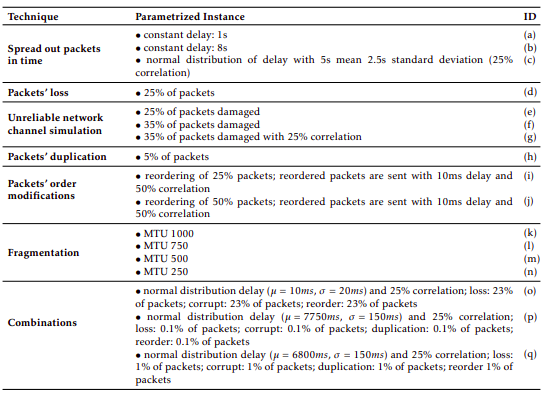
\includegraphics[scale=0.7]{img/asnm.png}
\captionof{figure}{Experimentelle Verschleierungstechniken mit Parametern und IDs \parencite{Homoliak2019}}\label{fig:asnm}
\end{center}
Das \ac{asnm} Datenset bietet ein ausführliches Featureset mit knapp 900 Attributen, allerdings verfügt es lediglich über knapp 7.000 Samples. Wie in Abschnitt \ref{asnm} beschrieben wurde dieses Set bereits von \textcite{Teoh2018} für die Analyse von Netzwerkverkehr verwendet.
\section{CERT}
\section{Ember}
\chapter{Prototypische Implementierung}
\chapter{Diskussion}
\chapter{Fazit}
\chapter{Zukünftige Forschung}
\newpage
%\frontmatter 
\pagenumbering{Roman}
\appendix
%\renewcommand{\refname}{Literaturverzeichnis}
%\bibliographystyle{plaindin}
%\bibliography{Bibtex/Masterarbeit-ma}
\printbibheading[heading=bibnumbered]
%
% einfache Möglichkeit der Trennung von Quellenarten via keyword
%
\printbibliography[notkeyword=internet, heading=subbibliography, %
   title={Bücher und Journals}]
\printbibliography[keyword=internet, heading=subbibliography, %
   title={Internetquellen}]
\renewcommand{\listfigurename}{Abbildungsverzeichnis}
\listoffigures
\renewcommand{\listfigurename}{}
\listoftables
\chapter{Abkürzungsverzeichnis}
\addcontentsline{toc}{section}{\textbf{Abkürzungsverzeichnis}}
\begin{acronym}
\acro{ab}[AB]{AdaBoost}
\acro{ack}[ACK]{acknowledge}
\acro{ann}[ANN]{Artificial Neural Network}
\acro{apts}[APTs]{Advanced Persistent Threats}
\acro{arff}[ARFF]{Attribute-Relation File Format}
\acro{asnm}[ASNM-NPBO]{Advanced Security Network Metrics \& Non-Payload-Based Obfuscations}
\acro{auc}[AUC]{Area Under the Curve}
\acro{aucroc}[AUC ROC]{area under the receiver operating characteristic curve}
\acro{awid}[AWID]{Aegean WiFi Intrusion Dataset}
\acro{bitkom}[BITKOM]{ Bundesverband Informationswirtschaft,Telekommunikation und neue Medien e.V.}
\acro{bka}[BKA]{Bundeskriminalamt}
\acro{bn}[BN]{Bayesian Network}
\acro{btb}[BTB]{Bug Terminating Bot}
\acro{cc}[C\&C]{Command \& Control}
\acro{cdns}[CDNs]{Content Distribution Networks}
\acro{cnn}[CNN]{Convolutional Neural Network}
\acro{cnns}[CNNs]{Convolutional Neural Networks}
\acro{crisp}[CRISP-DM]{Cross-Industry Standard Process for Data Mining}
\acro{c2}[C2]{Command and Control}
\acro{dbn}[DBN]{Deep Belief Network}
\acro{dbns}[DBNs]{Deep Belief Networks}
\acro{dpi}[DPI]{deep packet inspection}
\acro{dos}[DoS]{Denial of Service}
\acro{ddos}[DDoS]{Distributed Denial of Service}
\acro{dga}[DGA]{Domain Generation Algorithm}
\acro{dll}[DLL]{Dynamic Link Library}
\acro{dlls}[DLLs]{Dynamic Link Libraries}
\acro{dnn}[DNN]{Deep Neural Network}
\acro{dnns}[DNNs]{Deep Neural Networks}
\acro{dns}[DNS]{Domain Name System}
\acro{drbms}[DRBMs]{Deep Restricted Boltzmann Machines}
\acro{dt}[DT]{Decision Tree}
\acro{et}[ET]{Extra Random Trees}
\acro{fc}[FC]{Fuzzy Classifier}
\acro{fcn}[(FC) Neural Network]{Fully Connected Neural Network}
\acro{ff}[FF]{Fast-Flux}
\acro{fnr}[FNR]{False Negative Rate}
\acro{fpr}[FPR]{False Positive Rate}
\acro{ftp}[FTP]{File Transfer Protocol}
\acro{gbt}[GBT]{Gradient Boosting Tree}
\acro{gmm}[GMM-EM]{Gaussian-Mixture Model for Expectation-Maximization}
\acro{gnbt}[GNBT]{Gaussian Naive Bayes Tree}
\acro{gui}[GUI]{Graphical User Interface}
\acro{gpu}[GPU]{Graphics Processing Unit}
\acro{http}[HTTP]{Hypertext Transfer Protocol}
\acro{https}[HTTPS]{Hypertext Transfer Protocol Secure}
\acro{ibk}[IBk]{Instance-Based k}
\acro{icmp}[ICMP]{Internet Control Message Protocol}
\acro{ids}[IDS]{Intrusion Detection System}
\acro{imap}[IMAP]{Internet Message Access Protocol}
\acro{ioc}[IoC]{Indicator of Compromise}
\acro{iocs}[IoCs]{Indicators of Compromise}
\acro{iot}[IoT]{Internet of Things}
\acro{knn}[k-NN]{k-nearest-neighbor}
\acro{lanl}[LANL]{Los Alamos National Laboratory}
\acro{lb}[LB]{LogitBoost}
\acro{lddos}[LDDoS]{Low-rate DDoS}
\acro{lda}[LDA]{Linear Discriminant Analysis}
\acro{lgbm}[LightGBM]{Light Gradient Boosting Machine}
\acro{lr}[LR]{Logistic Regression}
\acro{lstm}[LSTM]{Long-Short Term Memory}
\acro{mlas}[MLAs]{Machine Learning Algorithmen}
\acro{mlp}[MLP]{Multi-Layer Perceptron}
\acro{nb}[NB]{Na\"ive Bayes}
\acro{nbt}[NBTree]{Na\"ive Bayesian Tree}
\acro{nlp}[NLP]{Natural Language Processing}
\acro{opcode}[Opcode]{Operation Code}
\acro{pe}[PE-Datei]{Portable Executable Datei}
\acro{pes}[PE-Dateien]{Portable Executable Dateien}
\acro{pop}[POP3]{Post Office Protocol v. 3}
\acro{psi}[PSI]{Printable String Information}
\acro{ram}[RAM]{Random-Access Memory}
\acro{rbm}[RBM]{Restricted Boltzmann Machine}
\acro{rnn}[RNN]{Recurrent Neural Network}
\acro{rnns}[RNNs]{Recurrent Neural Networks}
\acro{rf}[RF]{Random Forest}
\acro{rnnids}[RNN-IDS]{Recurrent Neural Networks für Intrusion Detection Systems}
\acro{r2l}[R2L]{Remote to Local}
\acro{smo}[SMO]{Sequential Minimal Optimization}
\acro{smtp}[SMTP]{Simple Mail Transfer Protocol}
\acro{ssh}[SSH]{Secure Shell}
\acro{svm}[SVM]{Support Vector Machine}
\acro{svms}[SVMs]{Support Vector Machines}
\acro{syn}[SYN]{synchronize}
\acro{tcp}[TCP]{Transmission Control Protocol}
\acro{tfidf}[TF-IDF]{Term Frequency - Inverse Document Frequency}
\acro{tpr}[TPR]{True Positive Rate}
\acro{udp}[UDP]{User Datagram Protocol}
\acro{u2r}[U2R]{User to Root}
\acro{vba}[VBA]{Visual Basic for Applications}
\acro{xgb}[XGBoost]{Extreme Gradient Boosting }
\acro{xss}[XSS]{Cross-Site Scripting}
\end{acronym}
%\end{document}
\newpage
\chapter{Anlagen}
\addcontentsline{toc}{section}{Anlagen}
\subsection*{Anlage 1: Research Model}\label{rm}

\begin{figure}[h!]
\hspace{-2.3cm}
%\begin{center}
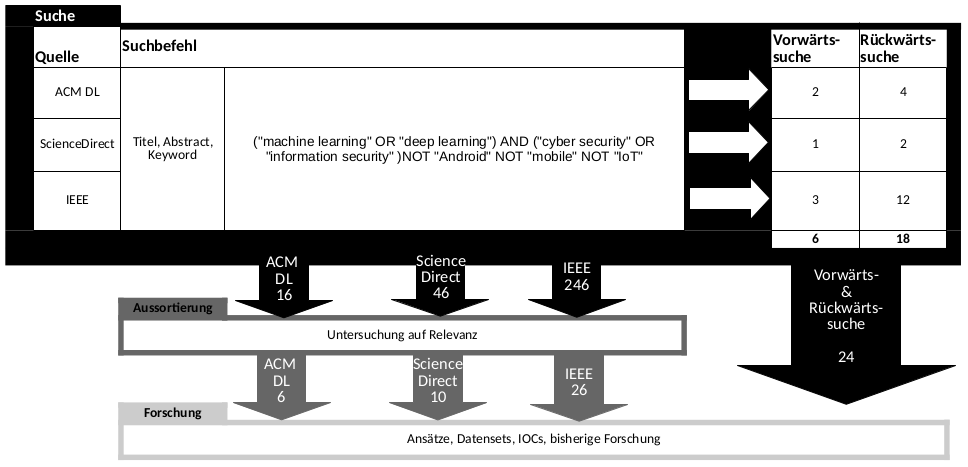
\includegraphics[width=1.3\textwidth]{img/rm}
\caption*{Prozess der Literaturrecherche}
%\end{center}
\end{figure}
\newpage
\subsection*{Anlage 2: Literaturreview}\label{literaturr}

\begin{figure}[h!]
\hspace{-2.2cm}
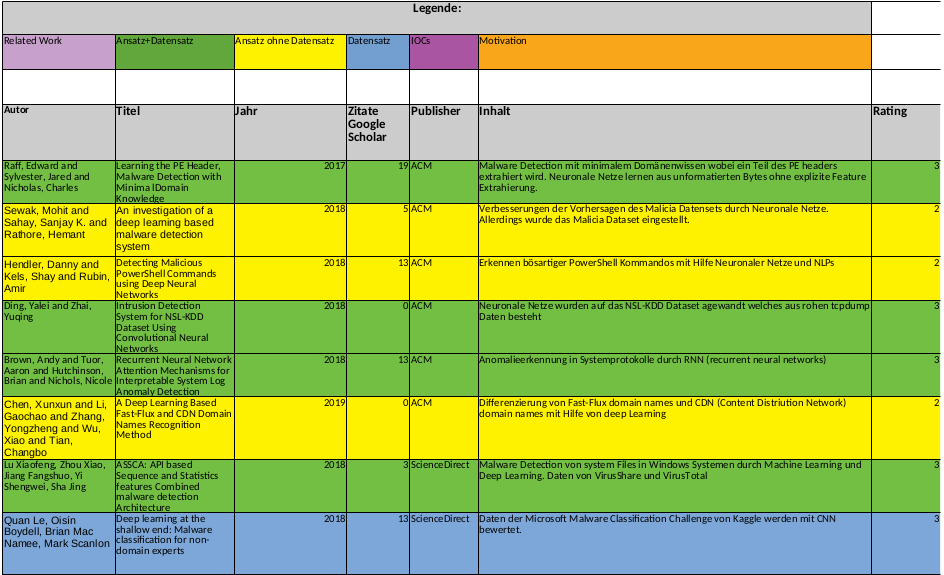
\includegraphics[width=1.3\textwidth]{img/literaturr}
\caption*{Ausschnitt der Literaturreview Liste}
\end{figure}
\listoftodos
\end{document}